%%%%%%%%%%%%%%%%%%%%%%% file template.tex %%%%%%%%%%%%%%%%%%%%%%%%%
%
% This is a general template file for the LaTeX package SVJour3
% for Springer journals.          Springer Heidelberg 2010/09/16
%
% Copy it to a new file with a new name and use it as the basis
% for your article. Delete % signs as needed.
%
% This template includes a few options for different layouts and
% content for various journals. Please consult a previous issue of
% your journal as needed.
%
%%%%%%%%%%%%%%%%%%%%%%%%%%%%%%%%%%%%%%%%%%%%%%%%%%%%%%%%%%%%%%%%%%%
%
\RequirePackage{fix-cm}
%
%\documentclass{svjour3}                     % onecolumn (standard format)
%\documentclass[smallcondensed]{svjour3}     % onecolumn (ditto)
\documentclass[natbib,smallextended]{svjour3}       % onecolumn (second format)
%\documentclass[twocolumn]{svjour3}          % twocolumn
%
\smartqed  % flush right qed marks, e.g. at end of proof
\bibliographystyle{aps-nameyear}
%
\usepackage{amsmath, amssymb}
\usepackage{graphicx}
\usepackage{amsfonts}
\usepackage{subcaption}
\usepackage{hyperref}
%\usepackage{pdflscape} % Landscape pages
\usepackage{color}	% Different font colors
\usepackage{enumerate}
\usepackage{enumitem}
\usepackage{mathtools}
\usepackage[]{algorithm2e}
\usepackage{color}
\usepackage{multirow} % Merging rows in tables
\usepackage{multicol} % Merging columns in tables
\usepackage{booktabs} % Horizontal rules in tables
\usepackage{mathrsfs} % Fancy math font for model labels
\usepackage{tikz}

\newcommand{\indentitem}{\setlength\itemindent{18pt}}
\renewcommand{\labelitemi}{$\bullet$}
\captionsetup{compatibility=false}
\newtheorem{prop}{Proposition}
\newtheorem{obs}{Observation}
\newtheorem{cor}{Corollary}
\newcommand\mycommfont[1]{\footnotesize\ttfamily\textcolor{blue}{#1}}
\SetCommentSty{mycommfont}
\SetKwRepeat{Do}{do}{while}
%
% \usepackage{mathptmx}      % use Times fonts if available on your TeX system
%
% insert here the call for the packages your document requires
%\usepackage{latexsym}
% etc.
%
% please place your own definitions here and don't use \def but
% \newcommand{}{} 
%
% Insert the name of "your journal" with
% \journalname{myjournal}
%
% original amsmath definition
% \subequations:
% \long macro:->\refstepcounter {equation}\protected@edef \theparentequation {\theequation }\setcounter {parentequation}{\value {equation}}\setcounter {equation}{0}\def \theequation {\theparentequation \alph {equation}}\ignorespaces 

% saved by hyperref in
% > \HyOrg@subequations=\long macro:

% hyperref-patched \subequations: (\endsubequations not modified)
% > \subequations=macro:
% ->\stepcounter {equation}\protected@edef \theHparentequation {\@ifundefined {th
% eHequation}\theequation \theHequation }\addtocounter {equation}{-1}\HyOrg@subeq
% uations \def \theHequation {\theHparentequation \alph {equation}}\ignorespaces 
% .


% extending the environment
%   1. with optional parameter: expected values resume or intermezzo or none.
%   2. while keeping the hyperref customization.

\makeatletter
\def\user@resume{resume}
\def\user@intermezzo{intermezzo}
%
\newcounter{previousequation}
\newcounter{lastsubequation}
\newcounter{savedparentequation}
\setcounter{savedparentequation}{1}
% 
% The following code causes that we are able to continue with numbering of a model in a next \align .
% For example:
%    a < b    (1a)
%    a < c    (1b)
% some text comes here and the numbering will continue:
%    a < d    (1c)
%
\renewenvironment{subequations}[1][]{%
      \def\user@decides{#1}%
      \setcounter{previousequation}{\value{equation}}%
      \ifx\user@decides\user@resume 
           \setcounter{equation}{\value{savedparentequation}}%
      \else  
      \ifx\user@decides\user@intermezzo
           \refstepcounter{equation}%
      \else
           \setcounter{lastsubequation}{0}%
           \refstepcounter{equation}%
      \fi\fi
      \protected@edef\theHparentequation{%
          \@ifundefined {theHequation}\theequation \theHequation}%
      \protected@edef\theparentequation{\theequation}%
      \setcounter{parentequation}{\value{equation}}%
      \ifx\user@decides\user@resume 
           \setcounter{equation}{\value{lastsubequation}}%
         \else
           \setcounter{equation}{0}%
      \fi
      \def\theequation  {\theparentequation  \alph{equation}}%
      \def\theHequation {\theHparentequation \alph{equation}}%
      \ignorespaces
}{%
%  \arabic{equation};\arabic{savedparentequation};\arabic{lastsubequation}
  \ifx\user@decides\user@resume
       \setcounter{lastsubequation}{\value{equation}}%
       \setcounter{equation}{\value{previousequation}}%
  \else
  \ifx\user@decides\user@intermezzo
       \setcounter{equation}{\value{parentequation}}%
  \else
       \setcounter{lastsubequation}{\value{equation}}%
       \setcounter{savedparentequation}{\value{parentequation}}%
       \setcounter{equation}{\value{parentequation}}%
  \fi\fi
%  \arabic{equation};\arabic{savedparentequation};\arabic{lastsubequation}
  \ignorespacesafterend
}
\makeatother

\begin{document}

\title{Integer Programming Formulations for the Shared Multicast Tree Problem
%\thanks{Grants or other notes
%about the article that should go on the front page should be
%placed here. General acknowledgments should be placed at the end of the article.}
}
% \subtitle{Tightening the LP bounds}
\titlerunning{IP formulations for SMT}        % if too long for running head

\author{Marika Ivanova        \and
         Dag Haugland
}
%\authorrunning{Short form of author list} % if too long for running head

\institute{M. Ivanova \at
              Department of Informatics, University of Bergen, Norway \\
              Tel.: +47 94277070\\
              \email{Marika.Ivanova@uib.no}         %  \\
%             \emph{Present address:} of F. Author  %  if needed
           \and
           D. Haugland \at
              Department of Informatics, University of Bergen, Norway \\
              Tel.: +47 55584033\\
              \email{Dag.Haugland@uib.no}         %  \\
}

\date{Received: date / Accepted: date}
% The correct dates will be entered by the editor
\maketitle

\begin{abstract}
We study the Shared Multicast Tree (SMT) problem in wireless networks.
To support a multicast session between a set of network nodes, SMT aims to establish a wireless 
connection between them, such that the total energy consumption is minimized.
All destinations of the multicast message must be connected, while non-destinations are optional nodes that can be used to relay messages. 
% MI: I believe these sentences can be disregarded, because the related problems are discussed in detail in the Introduction.
%In the well-studied minimum energy multicast (MEM)
%problem, the optimal tree depends on the source of the message.
%In contrast, SMT asks for a source-independent tree, which substantially reduces the processing overhead at each node.
%This means that SMT can be regarded as a Steiner tree problem.
%The objective function reflecting power consumption, however, distinguishes SMT clearly from the traditional minimum Steiner tree problem.
The objective function reflecting power consumption distinguishes SMT clearly from the traditional minimum Steiner tree problem.

%In the present work,
We develop two integer programming formulations for SMT.
Both models are subsequently extended and strengthened. % by redundant valid inequalities.
%Further strengthening is achieved by extending the set of variables and corresponding constraints.
Theorems on relations between the LP bounds corresponding to the models are stated and proved.
As the number of variables in the strongest formulations is a polynomial of degree four in the number of network nodes,
the models are impractical for computing lower bounds in instances beyond a fairly small size, 
%To make them applicable to larger instances, a constraint generation scheme is developed.
and therefore a constraint generation scheme is developed.
Results from computational experiments with the models demonstrate good promise of the approaches taken.
\keywords{Wireless communication, multicast tree, Steiner tree, LP bound, valid inequalities}
% \PACS{PACS code1 \and PACS code2 \and more}
% \subclass{MSC code1 \and MSC code2 \and more}
\end{abstract}

\section{Introduction}
\label{intro}

Wireless ad hoc networks (WANETs) are suitable in various practical applications in both civil and military sector, where a communication infrastructure is either absent or cannot be relied on.
Owing to their quick deployment and simple configuration, WANETs are useful in emergency operations such as natural disaster relief and military command and control.
Recently, the WANET concept has been introduced in ad hoc smart lighting in homes and in offices as well as ad hoc street light networks, where the control includes adjusting dimmable lights.
 
The purpose of a multicast communication session in a WANET is to route information from a sending device to a set of receiving devices.
Connection links are established by assigning sufficient power to the sending devices.
Since the devices typically use batteries as power supply, they are heavily energy-constrained.
Therefore, power efficiency is an important measure in designing WANETs.
Individual devices work as transceivers, which means that they have the ability to both transmit and receive a signal.
Moreover, the power level of a device can be dynamically adjusted during a multicast session.
\citet{montemanni11} name several applications of wireless sensor networks where power saving is essential.

Unlike wired networks, where signal passing takes place along predefined links, nodes in WANETs use omnidirectional antennas, and hence a message reaches all nodes within the communication range of its sender.
This range is determined by the power assigned to the sender, which is the maximum rather than the sum of the powers necessary to reach all intended receivers.
This feature is often referred to as the \emph{wireless advantage} \citep{Wieseltier00onthe}.

A well-known and extensively studied problem in the network design literature is the \textsc{Minimum Energy Broadcast} (MEB) problem.
Given a set of wireless devices with one designated source node, the goal is to assign powers to individual nodes.
The power assignments determine the communication ranges, and induce a broadcast tree such that a signal initiated by the source reaches, directly or via other nodes,
all the remaining nodes.
In the MEB problem, the task is to find power assignments enabling such a signal broadcast while minimizing the total energy consumption.
A natural and frequently addressed extension of MEB, is the \textsc{Minimum Energy Multicast} (MEM) problem.
Analogous to the difference between the \textsc{Minimum Spanning Tree} and the \textsc{Minimum Steiner Tree} problems,
MEM is distinguished from MEB in that not all nodes in the network are destinations of the multicast message.
Hence, the more general problem amounts to finding a Steiner tree spanning the destination nodes such that the sum of the power assignments is minimized.
Non-destination nodes are allowed in the Steiner tree, and will be included to the extent that they contribute to reduced power consumption.

In certain practical settings, MEB fails to reflect reality adequately.
Consider an application where more than one node can act as a source.
% Every node may initiate a message intended for the remaining nodes.
The optimal broadcast trees corresponding to two different sources are not necessarily identical,
and the optimal broadcast trees must be calculated separately for every possible source node.
In order to relay a received signal correctly, the nodes must be able to recognize which node initiated the received signal, and therefore also determine which broadcast tree to use.
Further, which power level to be set must be assessed by the relaying node.
Such overhead calculations require additional energy, and enabling the communication devices to accomplish them may even be impractical.

The idea behind the \textsc{Minimum Shared Broadcast Tree} (SBT) problem is to maintain a single, shared broadcast tree, to be applied regardless of which node is the signal source.
Such a tree is not necessarily optimal for any of the individual sources, but routing at each node is considerably simplified.
Provided that a shared broadcast tree is used, the nodes are no longer required to identify the source of the message in order to set a correct power level.
Instead, only the immediate neighbour from which the signal was received must be recognized.
The objective function in SBT captures not only the power levels of the nodes, but depends also on how frequently a node actually transmits with a certain power level.

Contributions from the present work include two sets of IP models for SMT, presented in order of increasing lower bounding capabilities.
By rigorous analysis of the models, we prove relations between the bounds offered by the corresponding continuous relaxations.
Intended for instances beyond the size that can be solved to optimality, we also develop a constraint generation procedure by which strong bounds can be computed.

The remainder of this paper is organized as follows: 
Section \ref{sec:literature} summarizes relevant literature and previous works.
%Section \ref{sec:SBT} describes the SMT problem and gives detailed explanation of its objective function.
Section \ref{sec:SBT} divided into three subsections introduces the notation, explains the network model, and gives formal definition of the problem.
Integer linear programming formulations, valid inequalities and their analysis are presented in Section \ref{sec:ILP},
followed by Section \ref{sec:comp}, where the models under study are compared with respect to strength.
In Section \ref{sec:strong}, the models are further extended by variables in higher dimensional spaces,
and a constraint generation procedure is developed.
Computational results are reported in Section \ref{sec:exp},
and suggestions to future work are summarized in Section \ref{sec:conclusion}.

\section{Literature Overview}
\label{sec:literature}

The combinatorial optimization literature is already rich on Integer Programming (IP) approaches to power minimization in wireless networks.
Since the work of \citet{Wieseltier00onthe}, in particular the MEB and MEM problems have been studied extensively.
Noteworthy contributions to this research include the IP models studied by \citet{das03},
\citet{altinkemer05}, \citet{yuan05}, \citet{yuan08}, \citet{bauer08}, \citet{montemanni11} and \citet{leggieri08}. 
\textcolor{blue}{
The latter paper proposes an IP formulation of MEM based on a Set Covering model together with a preprocessing procedure reducing the number of constraints.}
\citet{cagalj02} proved that MEB, and thereby MEM, is NP-hard.
Numerous contributions to fast, but possible inexact methods for MEM have thus appeared, and the interested reader is referred to \citep{hsiao13} for an overview. 
\textcolor{blue}{Another study concerning MEM is \cite{guo}, where the authors investigate energy conservation while using adaptive antennas. 
Unlike omnidirectional antennas, adaptive antennas can concentrate their transmission power in a smaller angle.}

\textcolor{blue}{\citet{bein10} study energy efficiency in wireless networks where all nodes can initiate a message, and the communicatin takes place in a single all-to-all broadcast tree.
A heuristic algorithm generating all-to-all broadcast trees is proposed in \citet{bhukya14}, along with an experimental evaluation confirming its merit.}

The SBT problem has also received some attention in the scientific literature.
It was introduced by \citet{Papadimitriou06SBT}, who also proved that the problem is NP-hard.
In the same article, an approximation algorithm for SBT was developed and analyzed experimentally.
Building on this work, \citet{Haugland12Dual} presented an integer programming model for SBT, along with an associated decomposition approach.

Simple instances \citep{Haugland12Dual} show that because of the difference in objective functions, the optimal solutions to RAP and SBT can differ substantially.
\citet{kirousis97} and \citet{clementi99} conduct
hardness results for instances of RAP embedded in three- and two-dimensional Euclidean space, respectively.
Later, IP models have been developed by e.g.\ \citet{althaus03}, \citet{montemanni04}, \citet{das05}, and \citet{Haugland11Compact}.

Some preliminary work on SMT has recently been published.
\citet{ivanova16isco} introduces the problem, and develops an IP model.
Moreover, the author studies inexact construction and improvement methods, for which computational results are reported.

\section{The Minimum Shared Multicast Tree Problem}
\label{sec:SBT}
Like in studies of other problems in combinatorial optimization,
a theoretical investigation of SMT requires abstraction and simplification of the real-world communication network.

\subsection{Assumptions and notation} \label{sec:notation}

A WANET is modeled by a complete graph $G=(V,E)$, where the set $V$ of nodes represents the set of wireless devices,
and the set of edges $E=\{\{i,j\}:i,j\in V, i\neq j\}$ corresponds to the potential links between them.
The set $A=\{(i,j):i,j\in V,\{i,j\}\in E\}$ consists of all arcs that can be derived by directing the edges in $E$.
Nodes in the set $D\subseteq V$ are the destination nodes, also referred to as \emph{source} nodes.
For an arbitrary $i\in V$, sets $V\setminus \{i\}$ and $D\setminus\{i\}$ are denoted $V_i$ and $D_i$, respectively.

Sending a message directly from (to) node $i$ to (from) node $j$ requires a positive \emph{transmission power} $p_{ij}=p_{ji}$.
Whenever appropriate, $p_{ij}$ is referred to as the \emph{cost} of $\{i,j\}$,
and edges with higher cost than others are said to be \emph{more expensive}.
When the nodes are embedded in the plane, $p_{ij}$ is often assumed \citep{Papadimitriou06SBT,Haugland12Dual,halgamuge} to be
proportional to the Euclidean distance between $i$ and $j$ raised to a power between 2 and 4.
For simplicity, we assume for all $i\in V$ that $p_{ij}\neq p_{ik}$ when $j\neq k$, and define
$W_{ij}=\left\{k\in V_i: p_{ik}\geq p_{ij}\right\}$
as the set of nodes requiring no less power at $i$ than $j$ does.
The notation $G'\subseteq G$ means that $G'=(V_{G'},E_{G'})$ is a subgraph of $G$, 
i.e., $E_{G'}\subseteq E$ consists uniquely of edges in $E$ with both end nodes in $V_{G'}\subseteq V$.

Let $y \in \{0,1\}^E$ and $X\in\{0,1\}^{A\times D}$ be binary vectors with components corresponding to edges,
and pairs of arcs and destination nodes, respectively.
The vector $X^s$ then consists of all components of $X$ corresponding to a pair of which $s$ is the destination.
The subgraph of $G$ \emph{induced by} $y$ is defined as $G_y=(V,E_y)$, where $E_y=\left\{\{i,j\}\in E: y_{ij}=1\right\}$.
Directed graphs induced by binary vectors over $A$ are defined analogously.

Several integer programming models, all of which exclusively have binary variables, will be considered in this text.
If $\mathcal{M}$ is such a model, $\text{LP}(\mathcal{M})$ denotes the corresponding continuous relaxation
where the domain of each variable is replaced by the interval $[0,1]$.
Further, $z\left(\mathcal{M}\right)$ and $z\left(\text{LP}(\mathcal{M})\right)$ denote the optimal objective function values of the respective models.


\subsection{Network model} \label{sec:netmod}

To illustrate the problem under study, consider the tree depicted in Fig. \ref{fig:objexp}.
Seven destination nodes ($D=\{i_1,i_2,a,b,c,d,e\}$) are spanned by use of two Steiner nodes ($V\setminus D = \{i,i_3\}$).
Consider node $i$ and its three neighbour nodes $i_1$, $i_2$ and $i_3$, ordered by decreasing power requirement at $i$.
That is, $p_{ii_1}>p_{ii_2}>p_{ii_3}$.
If the transmitting node is outside the shaded area ($i_2$, $c$, $d$, or $e$), then node $i$ relays the signal to two of its neighbors, \emph{including $i_1$}.
Exploiting the wireless advantage, the signal from node $i$ reaches both neighbors if it is assigned power level $p_{ii_1}$.
Otherwise, if the signal source is either $i_1$, $a$, or $b$, node $i$ passes the signal on to neighbors $i_2$ and $i_3$.
This is accomplished by setting the power level of $i$ to $p_{ii_2}$.

\begin{figure}[h!]
\centering
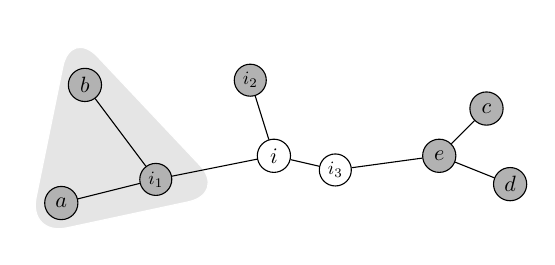
\begin{tikzpicture}[scale=.6]
 \draw[rounded corners=5mm, fill=gray!20, draw=white] (-.7,-.2) -- (3.5,0.7) -- (0.2,4.2) -- cycle;
 \begin{scope}[every node/.style={circle,draw=black,fill=gray!60,minimum size=1.5em, inner sep=2, scale=.8}]
  \node (a) at (0,0.5) {$a$};
  \node (b) at (0.5,3) {$b$};
  \node (c) at (9,2.5) {$c$};
  \node (d) at (9.5,0.9) {$d$};
  \node[scale=.85] (i1) at (2,1) {$i_1$};
  \node[scale=.85] (i2) at (4,3.1) {$i_2$};
  \node[scale=.85,fill=none] (i3) at (5.8,1.2) {$i_3$};
  \node[fill=none] (i) at (4.5,1.5) {$i$};
  \node (e) at (8,1.5) {$e$};
 \end{scope}
 \draw (a) -- (i1) -- (b);
 \draw (i1) -- (i) -- (i3) -- (e) -- (c);
 \draw (e) -- (d);
 \draw (i) -- (i2);
\end{tikzpicture}
\caption{A multicast tree illustrating the cost contribution from node $i$ to the objective function.
	 Destinations and Steiner nodes are denoted by filled and empty circles, respectively.}
\label{fig:objexp}
\end{figure}

In more general terms, let $T\subseteq G$ be a multicast tree, and let $i\in V_T$ be a node with at least two neighbors in $T$.
For multicasting a message, the power to be assigned to node $i$ is either $p_{ii_1}$ or $p_{ii_2}$, where $i_1$ and $i_2$ are neighbors of $i$ such that
$p_{ii_1}>p_{ii_2}>p_{ij}$ for all other neighbors $j\neq i_1,i_2$ of $i$ in $V_T$.
If the path from the message source to $i$ intersects $i_1$, then power $p_{ii_2}$ is sufficient.
Otherwise, the power $p_{ii_1}$ is required.
At a leaf $i$ with neighbor $i_1$ in $T$, the power assignment is $p_{ii_1}$ if $i$ also is the message source, and zero otherwise.

All nodes in $D$ are assumed to be equally likely to initiate a message.
The frequency at which power levels $p_{ii_1}$ and $p_{ii_2}$ (let $p_{ii_2}=0$ if $i$ is a leaf) are required,
is thus proportional to the number of sources in $D$ that utilize the respective arc for message forwarding.
In the example in Fig.\ \ref{fig:objexp}, the expected power consumption at node $i$ is thus proportional to $4p_{ii_1} + 3p_{ii_2}$.
Summing over all nodes yields the total cost of the tree.

The cost model outlined above aims for minimization of the transmission energy.
As pointed out by \citet{halgamuge}, transmission constitutes a substantial part of the total energy consumption in wireless sensor networks.
The energy consumed by other operations, such as sensing, logging, processing, actuation, and cluster formation is less sensitive to the topology
of the multicast tree, and is neglected in the current work.
This is in line with the approach taken in the wide range of literature on optimization models for wireless networks mentioned in Section \ref{sec:literature}.
For a detailed energy model for wireless sensor networks, the reader is referred to the article by \citet{halgamuge}.

\subsection{Problem definition} \label{sec:probdef}

To express the cost of the multicast tree more rigorously, let $T^s=(V_T,A^s)$ denote the directed tree (arborescence) obtained by directing all edges in $T$ such that they point away from the \emph{root} at $s$.
For each arc $(i,j)\in A$, we let $n_{ij}(T)$ denote the number of destinations $s$ such that $(i,j)$ is the most expensive arc leaving node $i$ in $T^s$.
That is,
\[
  n_{ij}(T) = \left|\left\{s\in D: p_{ij}=\max_{k\in V_i: (i,k)\in A^s}p_{ik}\right\}\right|,
\]

\noindent
and the total cost of tree $T$ becomes:
$$
  c(T) = \sum_{i\in V_T}\sum_{j\in V_T:\{i,j\}\in E_T}p_{ij}n_{ij}(T).
$$ 
The problem under study is thus defined in network optimization terms:

\begin{problem}
\label{def:problem}
\textsc{Minimum Shared Multicast Tree}: Find a tree $T\subseteq G$ spanning $D$ such that $c(T)$ is minimized.
\end{problem}

While the feasible domains of the \textsc{Minimum Steiner Tree} problem and SMT are identical,
the cost functions differ.
In the former problem, all edges present in the tree contribute to the objective function by a cost that is given by the input data.
The input cost factor $p_{ij}$ is, in the case of SMT, scaled by a topology dependent factor $n_{ij}(T)$.
Only edges that are the most or second-most expensive edge incident to either of their end nodes get a positive scaling factor.
Some edges in $T$ can thus be scaled down to zero cost, while the most expensive ones are scaled up.

Problem \ref{def:problem} also has close resemblance with the SBT problem, which is the special case of SMT where $D=V$.
Like many other network design problems, SMT is NP-hard.
This follows directly from the NP-hardness of SBT \citep{Papadimitriou06SBT}.


In the forthcoming sections, we develop and analyze IP models for SMT.
All formulations under study are extensions of models previously developed for the related problems mentioned above.

\section{IP Formulations}
\label{sec:ILP}

A basic element of every IP formulation for SMT is a set of constraints modelling a Steiner tree.
We investigate two such constraint sets formulated in terms of variables with up to three node indices, and make necessary extensions required by the objective function of SMT.
The resulting models are subsequently strengthened by valid inequalities.

\subsection{Formulation based on broadcast trees}

The first model extends the SBT formulation introduced by \citet{Haugland12Dual} by non-destination nodes, in order to formulate the multicast version of the problem \citep{ivanova16isco}.

\subsubsection{Underlying Steiner tree formulation}

Feasible solutions to SMT are characterized by a Steiner tree $T$ covering $D$.
Define for each edge $\{i,j\}\in E$ and each destination node $s\in D$, the binary variables $y\in\{0,1\}^E$ and $X\in\{0,1\}^{A\times D}$,
where $y_{ij}=1$ iff $\{i,j\} \in E_T$,
and $X^{s}_{ij}=1$ iff $(i,j)\in A^s$.
% \[y_{ij}=
% \begin{cases}
%     1 & \text{if $\{i,j\} \in E_T$},\\
%     0 & \text{otherwise},
%   \end{cases}
% \]
% 
% \[X^{s}_{ij}=
% \begin{cases}
%     1 & \text{if $(i,j)$ is an arc in the arborescence $T^s$},\\
%     0 & \text{otherwise}.
%   \end{cases}
% \]
To induce a graph with an acyclic connected component spanning $D$, the following constraints are imposed:
%%%%%%%%%%%%%%%%%%%%%%%%%%%%%%%%%%%%%%%
%                                     % 
%     STEINER TREE MODEL  X0          %
%                                     %
%%%%%%%%%%%%%%%%%%%%%%%%%%%%%%%%%%%%%%%
\begin{subequations}\label{mod:x0}
\begin{align}
\label{con:dd:arrowFromDest} \sum\limits_{j\in V_i}X^s_{ji} & = 1 & i,s\in D,i\neq s,\\
\label{con:dd:arrowFromNonDestB} \sum\limits_{j\in V_{i}}X^s_{ji} & \leq 1 & i\in V \setminus D, s\in D,\\
\label{con:dd:arrowFromNonDestA} X^s_{ij} & \leq \sum\limits_{k\in V_{i}\setminus \{j\}}X^s_{ki} & i\in V \setminus D,(i,j)\in A, s\in D,\\
\label{con:dd:oneDir} X^s_{ij} + X^s_{ji} & = y_{ij} & \{i,j\}\in E, s\in D,\\
\label{con:dd:startInSource} X^s_{is} & = 0 &  s\in D, (i,s)\in A,&\\
\label{con:dd:vardim}y \in \{0,1\}^{E}, X & \in \{0,1\}^{A\times D}.
\end{align}~
\end{subequations}

Constraints (\ref{con:dd:arrowFromDest}) ensure that all destination nodes but $s$ have a unique entering arc in $T^s$.
Inequalities (\ref{con:dd:arrowFromNonDestB})--(\ref{con:dd:arrowFromNonDestA})
say that non-destination nodes do not have more than one entering arc, and that they do have one if they have leaving arcs.
Constraints (\ref{con:dd:oneDir}) state that the arc set of $T^s$ consists of directed versions of the edge set of $T$,
and (\ref{con:dd:startInSource}) ensure that $s$ is the root of $T^s$.
More formally, the effect of the constraints can be stated as follows:

\begin{lemma} \label{lem:x0valid}
If $(X,y)$ satisfies (\ref{con:dd:arrowFromDest})--(\ref{con:dd:vardim}), then $G_y$ has a tree spanning $D$ as one of its connected components.
Conversely, for any tree $T\subseteq G$ spanning $D$, there exists a pair $(X,y)$ satisfying (\ref{con:dd:arrowFromDest})--(\ref{con:dd:vardim}) such that $T$
is a connected component of $G_y$.
\end{lemma}
\begin{proof}
By (\ref{con:dd:startInSource}) and (\ref{con:dd:arrowFromDest})--(\ref{con:dd:arrowFromNonDestB}),
the in-degree of $s\in D$ is 0 in $G_{X^s}$, whereas it is at most one at all other nodes.
Hence, the connected components of $G_{X^s}$ are directed cycles, arborescences, and isolated nodes,
and one of the components is an arborescence rooted at $s$.
Constraints (\ref{con:dd:oneDir}) imply that $G_y$ consists of undirected versions of the same components,
showing that no cycle in $G_y$ contains destination nodes.
Let $t\in D$, and let $P$
be the maximal path in $G_{X^s}$ that terminates in $t$.
Existence and uniqueness of this path is assured since $t$ belongs to an acyclic connected component.
According to (\ref{con:dd:arrowFromNonDestA}), each non-destination in $P$ has an entering arc in $P$,
while (\ref{con:dd:arrowFromDest}) ensures that the same is true for every destination node, except $s$.
It follows that the first node of $P$ is $s$.
Thus, destinations $s$ and $t$ belong to a joint, acyclic connected component of $G_y$.

The second claim of the lemma is obvious.\qed
\end{proof}


\subsubsection{SMT model [$\mathcal{X}_1$]} \label{sec:x1}

To reflect that only expensive edges in $T$ contribute to the objective function of Problem \ref{def:problem}, we introduce the variables:
\newline\newline
$\pi^s_{ij}=
\begin{cases}
    1 & \text{if $(i,j)$ is the most expensive arc leaving node $i$ in $T^s$},\\
    0 & \text{otherwise},
  \end{cases}$
\newline\newline
leading to the following formulation $\mathcal{X}_1$ of SMT:

%%%%%%%%%%%%%%%%%%%%%%%%%%%%%%%%%%%%%%%
%                                     % 
%             MODEL X1                %
%           (3 idx vars)              %
%%%%%%%%%%%%%%%%%%%%%%%%%%%%%%%%%%%%%%%
\begin{subequations}[resume]\label{eq:smt-x2}
\begin{align}
\label{objective:mf} \makebox[0pt][l]{$\displaystyle{} \min \sum\limits_{(i,j) \in A} p_{ij} \sum\limits_{s \in D} \pi^s_{ij} $}\\
\notag\text{s.t.}\\
\notag(\ref{con:dd:arrowFromDest}) &- (\ref{con:dd:vardim})\\
\label{con:dd:yvar} X^s_{ij} & \leq \sum_{k\in W_{ij}}\pi^s_{ik} & s\in D, (i,j)\in A,\\
\label{con:dd:vardimy} \pi & \in \{0,1\}^{A\times D}.
\end{align}~
\end{subequations}

Constraints (\ref{con:dd:yvar}) say that if $(i,j)\in A_{T^s}$, then the cost of the most expensive arc in $T^s$ leaving $i$ is at least $p_{ij}$.
Since $\sum_{s\in D}\pi_{ij}^s=n_{ij}(T)$ is the number of arborescences in which $(i,j)$ is the most expensive arc leaving $i$,
(\ref{objective:mf}) thus agrees with the objective of Problem \ref{def:problem}.

\begin{prop}
\label{prop:x1valid}
If $(X,y,\pi)$ is an optimal solution to $\mathcal{X}_1$, then $G_y$ consists of isolated non-destination nodes and a tree that
solves Problem \ref{def:problem}.
\end{prop}
\begin{proof}
Follows directly from $p\geq 0$ and Lemma \ref{lem:x0valid}.
\qed
\end{proof}

Model $\mathcal{X}_1$ is a slightly modified version of the SMT model introduced by \citet{ivanova16isco},
which contains a set of constraints disallowing non-destination leaves, and a weaker version of constraints (\ref{con:dd:arrowFromNonDestA}).
Formulation (\ref{objective:mf})--(\ref{con:dd:vardimy}) is \emph{minimal},
in the sense that each set of constraints is necessary in order to give a valid formulation.
In the next section, we strengthen the formulation by adding redundant valid inequalities.

\subsubsection{Valid inequalities [$\mathcal{X}_2$]} \label{sec:x2}

Adding the following valid inequalities to $\mathcal{X}_1$ gives another SMT-model, denoted $\mathcal{X}_2$:
%%%%%%%%%%%%%%%%%%%%%%%%%%%%%%%%%%%%%%%
%                                     % 
%             MODEL X2                %
%      (3 idx vars + VIs )            %
%%%%%%%%%%%%%%%%%%%%%%%%%%%%%%%%%%%%%%%
\begin{subequations}[resume]
\begin{align}
\label{con:dd:extraCon} \sum\limits_{j\in V_{i}}X^s_{ji} & \leq \sum\limits_{j\in V_{i}}X^s_{ij}  & 	i\in V\setminus D, s\in D,\\
\label{con:vi:Y1} \sum\limits_{j\in V_s}  \pi^{s}_{sj} & =1 & s\in D,\\
\label{con:vi:sumYImpSumX} \sum\limits_{j\in V_i\setminus\{s\} }\pi^{s}_{ij} & = \sum\limits_{j\in V_i}  X^{s}_{ji} & i\in V\setminus D, s\in D.
\end{align}
\end{subequations}
Constraints (\ref{con:dd:extraCon}) ensure that the number of arcs leaving a non-destination in $T^s$ is no less than the number of entering arcs.
Their effect is to disallow non-destination leaves.
Equations (\ref{con:vi:Y1}) say that in arborescence $T^s$, exactly one arc $(s,j)$ leaving the root $s$ is declared to be largest.
Validity of the constraints follows immediately because the root has at least one leaving arc.
As constraints (\ref{con:vi:sumYImpSumX}) state, if an arc enters non-destination node $i$ in $T^s$, then $i$ also has at least one out-going arc,
exactly one of which is the most expensive.
The root $s$ is excluded from the summation set on the left of (\ref{con:vi:sumYImpSumX}) since no arcs in $T^s$ enter $s$.

\begin{remark} \label{rem:x2}
The sets (\ref{con:dd:extraCon})--(\ref{con:vi:sumYImpSumX}) of valid inequalities are \emph{independent} in the following sense:
There exist instances where the removal of either set implies that $z(\text{LP}(\mathcal{X}_2))$ takes a smaller value.
This includes the instance where $|V|=9$, $|D|=5$, all power requirements (arc costs) $p_{ij}$ equal the square of the Euclidean distance between nodes $i$ and $j$,
and the nodes are located in the plane with respective coordinates (destinations mentioned first)
(47, 65), (8, 65), (26, 12), (78, 27), (8, 8), (73, 66), (13, 55), (91, 44), and (76, 74).
\end{remark}

\subsection{Formulation based on network flows}

There are many formulations for the \textsc{Minimum Steiner Tree} problem \citep{goemans93catalog} that can serve as a basis for modelling SMT.
We consider the multi-commodity network flow model developed by \citet{Polzin} (denoted $P_{F}$ in their work).
A given destination $s_0\in D$ plays a particular role in the models.
For the sake of simplified notation, $s_0$ as subscript (superscript) is henceforth replaced by subscript (superscript) 0.

\subsubsection{Underlying Steiner tree formulation}

To identify a Steiner arborescence $T^0=(V^0,A^0)$ rooted at $s_0$, we define variables $g\in\{0,1\}^A$ and $F\in\{0,1\}^{A\times D_0}$,
where $g_{ij}=1$ iff $(i,j)\in A$, and $F_{ij}^s=1$ iff  the path in $T^0$ from $s_0$ to destination $s$ contains arc $(i,j)$.
% the following variables are introduced for each arc $(i,j)\in A$ and destination $s\in D_0$:
% \newline\newline
%   $g_{ij}=
% \begin{cases}
%     1 & \text{if $(i,j) \in A^0$},\\
%     0 & \text{otherwise},
% \end{cases}$
% \newline\newline
%   $F^{s}_{ij}=
% \begin{cases}
%     1 & \text{if the path from $s_0$ to $s$ in $T^0$ contains $(i,j)$},\\
%     0 & \text{otherwise}.
% \end{cases}$
% \newline\newline
%
Variables $g_{ij}$ and $F_{ij}^s$ are traditionally referred to as the \emph{design variable} of arc $(i,j)$ and the
\emph{flow of commodity $s$} along $(i,j)$, respectively.
The constraints of the \emph{multi-commodity flow formulation}
of the \textsc{Minimum Steiner Tree} problem are:
%%%%%%%%%%%%%%%%%%%%%%%%%%%%%%%%%%%%%%%
%                                     % 
%     STEINER ARBORESCENCE F0         %
%        (from Polzin)                %
%%%%%%%%%%%%%%%%%%%%%%%%%%%%%%%%%%%%%%%
\begin{subequations}
\begin{align}
\label{con:pf1:xfrel} F^{s}_{ij} & \leq g_{ij} & s\in D_0, (i,j)\in A, \\
\label{con:pf1:flow} \sum\limits_{\substack{ j \in V_i }}F^{s}_{ji}-\sum\limits_{\substack{j\in V_i}}F^{s}_{ij} &= 
  \begin{cases}
    1, & i=s,\\
    0, & i\in V\setminus \{s_0, s\},
  \end{cases} & s\in D_0,\\
\label{con:pf1:B}  \sum_{j\in V_i}g_{ji}&\leq 1 & i\in V\setminus D,\\
\label{con:pf1:noflowFromT} F_{si}^s&=0 & s\in D_0, i\in V_s,\\
\label{con:pf1:fitt=xit} F_{is}^s&=g_{is} & s\in D_0, i\in V_s,\\
\label{con:pf1:xi0=0} g_{i0}&=0 & i\in V_0,\\
\label{con:pf1:dim}g \in \{0,1\}^{A},F&\in\{0,1\}^{A \times D_0}.
\end{align}~
\end{subequations}

The \emph{flow conservation} constraints (\ref{con:pf1:flow}) ensure that $T^0$ is connected,
and the \emph{capacity} constraints (\ref{con:pf1:xfrel}) state that flow of any commodity is allowed only if $(i,j)\in A^0$.
Multi-commodity flow formulations appear abundantly in the network design literature, and proof of the following claim is therefore omitted:

%%%%%%%%%%%%%%%%%%%%%%%%%%%%%%%%%%%%%%%
%                                     %
%         Proposition  		      %
% (F1 models an arborescence)         %
%                                     %
%%%%%%%%%%%%%%%%%%%%%%%%%%%%%%%%%%%%%%%
\begin{lemma}
\label{lem:modelcorrect}
Assume $(F,g)$ satisfies (\ref{con:pf1:xfrel})--(\ref{con:pf1:dim}).
Then some connected component $T^0\subseteq G_{g}$ is an $s_0$-rooted arborescence spanning $D$,
and some connected component of $G_{F^s}\subseteq T^0$ is a path from $s_0$ to $s\in D_0$.
Conversely, for any $s_0$-rooted arborescence $T^0$ spanning $D$, there exists a pair $(F,g)$ satisfying (\ref{con:pf1:xfrel})--(\ref{con:pf1:dim}) such that $T^0$
is a connected component of $G_g$.
\end{lemma}
 
To model the objective function of SMT, the following result is useful:
%%%%%%%%%%%%%%%%%%%%%%%%%%%%%%%%%%%%%%%
%                                     %
%         Proposition  		      %
%   (transformation X_{ij}^s)         %
%                                     %
%%%%%%%%%%%%%%%%%%%%%%%%%%%%%%%%%%%%%%%
\begin{prop}\label{prop:transx}
Assume $(F,g)$ satisfies (\ref{con:pf1:xfrel})--(\ref{con:pf1:dim}),
and let $T^s=(V^s,A^s)$ be the arborescence obtained by redirecting the arcs in $T^0$ such that they point away from $s\in D_0$. Then
$$
g_{ij} - F^s_{ij}+F^s_{ji} = 
	\begin{cases}
		1, ~\text{if $(i,j)\in A^s$}, \\
		0, ~\text{otherwise.}
	\end{cases}
$$
\end{prop}
%
\begin{proof}
Because $T^0$ is acyclic, it follows from the capacity constraints (\ref{con:pf1:xfrel}) that $g_{ij}+F^s_{ji}\leq 1$.
The same constraints also imply $g_{ij} - F^s_{ij}\geq 0$.
Hence, $g_{ij} - F^s_{ij}+F^s_{ji}\in\{0,1\}$.

Arborescence $T^s$ contains arc $(i,j)$ iff $(i,j)$ is in $A^0$ but not on a path to $s$, or its reverse arc $(j,i)$ is on such a path.
By Lemma \ref{lem:modelcorrect}, this disjunction is equivalent to $g_{ij}-F_{ij}^s=1$ or $F_{ji}=1$.
The result then follows since the two conditions are mutually exclusive.
\qed
\end{proof}

% $\mathcal{F}_1$ based on $\mathcal{F}_0$.
% For this purpose, it is necessary to find a way to represent the constraint (\ref{con:dd:yvar}) in the $\mathcal{F}_1$ space.
% The $\pi$-variables from $\mathcal{X}_1$ have to be used in $\mathcal{F}_1$, because they appear in the objective function which remains unchanged.

\subsubsection{SMT model [$\mathcal{F}_1$]}

Recall from Section \ref{sec:x1} that $\pi_{ij}^s$ determines whether $(i,j)$ is the most expensive arc leaving node $i$ in arborescence $T^s$.
Taking advantage of Prop.\ \ref{prop:transx}, we can thus formulate Problem \ref{def:problem} in terms of variables $F$, $g$, and $\pi$,
resulting in model $\mathcal{F}_1$:
%%%%%%%%%%%%%%%%%%%%%%%%%%%%%%%%%%%%%%%
%                                     % 
%             MODEL F1                %
%        (3 idx vars)                 %
%%%%%%%%%%%%%%%%%%%%%%%%%%%%%%%%%%%%%%%
\begin{subequations}[resume]
\begin{align}
\notag\min & \sum\limits_{(i,j) \in A} p_{ij} \sum\limits_{s \in D} \pi^s_{ij}\\ 
\notag\text{s.t.} && \\
\notag(\ref{con:pf1:xfrel}) - (\ref{con:pf1:dim})\\
\label{con:pf1:yvar} g_{ij} - F^s_{ij}+F^s_{ji} & \leq \sum_{k\in W_{ij}}\pi^s_{ik}  & s\in D_0, (i,j)\in A,\\
\label{con:pf1:yvar0} g_{ij} & \leq \sum_{k\in W_{ij}}\pi^0_{ik}   &  (i,j)\in A,\\
\label{con:pf1:dimy} \pi&\in \{0,1\}^{A\times D}.
\end{align}~
\end{subequations}

Like (\ref{con:dd:yvar}), constraints (\ref{con:pf1:yvar}) ensure that if $(i,j)\in A^s$, then $\pi_{ik}^s=1$ for some
arc $(i,k)$ at least as expensive as $(i,j)$.
As $g_{ij}$ determines whether $(i,j)\in A^0$, the corresponding constraint for destination $s_0$ is simplified to (\ref{con:pf1:yvar0}).
Validity of $\mathcal{F}_1$ is thus stated as a corollary to Prop.\ \ref{prop:transx}:

\begin{cor}
If $(F,g,\pi)$ is an optimal solution to $\mathcal{F}_1$, then $G_g$ consists of isolated non-destination nodes and an arborescence $T^0$.
The tree obtained by disregarding arc directions in $T^0$ is an optimal solution to Problem \ref{def:problem}.
\end{cor}

\begin{remark} \label{rem:f1a}
Like $\mathcal{X}_1$, also $\mathcal{F}_1$ is a minimal formulation.
Constraints (\ref{con:pf1:B}) prevent non-destinations from having multiple entering arcs.
In a \textsc{Minimum Steiner Tree} formulation, where a linear function of $g$ is minimized subject to constraints
(\ref{con:pf1:xfrel})--(\ref{con:pf1:flow}) and (\ref{con:pf1:noflowFromT})--(\ref{con:pf1:dim}),
constraints (\ref{con:pf1:B}) are implied by optimality.
The necessity of (\ref{con:pf1:B}) in formulation $\mathcal{F}_1$ of SMT is demonstrated by the optimal solution to $\mathcal{F}_1$ after removal of (\ref{con:pf1:B})
in the following instance: $V=\{s_0,a,\ldots,i\}$ with coordinates
(3, 61),
(79, 80),
(32, 54),
(93, 21),
(12, 70),
(93, 60),
(72, 78),
(76, 80),
(39, 84), and
(82, 80), respectively, edge costs equal to the square of the Euclidean distance between end points, and $D=\{s_0,a,\ldots,f\}$.
Figure \ref{fig:BProof} depicts the optimal solution to SMT, and the solution to $\mathcal{F}_1$ after removal of (\ref{con:pf1:B}).
%The optimal solution with objective value 25156 to the depicted instance obtained by solving SMT-$\mathcal{X}_1$ is shown in Fig. \ref{fig:BorigSMT}.
%The solution in Fig \ref{fig:Bpf2} yielded by solving SMT-$\mathcal{F}_1$ without the constraint (\ref{con:pf1:B}) has objective value 25148, but is not a feasible solution to Problem \ref{def:problem}, because of the cycle $(g,h,i,d,g)$.
%The non-existence of such a cycle in a solution given by model $\mathcal{X}_1$ is ensured by constraints (\ref{con:dd:arrowFromDest}), (\ref{con:dd:arrowFromNonDestB}) and (\ref{con:dd:oneDir}).
%A detailed proof of this claim can be found in \cite{ivanova16isco}.
%A transmission commenced in node $c$ is sent via arc $(g,f)$.
%As a consequence of the link between $g$ and $d$ in Fig. \ref{fig:Bpf2}, the node $d$ also receives the message.
%This link is absent in Fig. \ref{fig:BorigSMT}, and so $i$ has to relay the signal using arc $(i,d)$, causing the higher total objective value.
\end{remark}
\begin{remark} \label{rem:f1b}
The obviously valid inequalities (\ref{con:pf1:noflowFromT})--(\ref{con:pf1:fitt=xit}) are not necessary in the \textsc{Minimum Steiner Tree} formulation,
but have to be included in the formulation $\mathcal{F}_1$ of SMT in order to disallow nodes in $D_0$ to have multiple entering arcs.
Removal of (\ref{con:pf1:noflowFromT}) or (\ref{con:pf1:fitt=xit}) implies that the optimal solution to the instance where
$V=\{s_0,a,\ldots,k\}$ with coordinates
(43, 15),
(89, 88),
(56, 12),
(44, 66),
(60, 42),
(91, 48),
(64, 8),
(64, 34),
(68, 9),
(41, 53),
(85, 67), and
(93, 49), respectively,
edge costs defined as in Remark \ref{rem:f1a}, and $D=\{s_0,a,\ldots,h\}$,
is not a feasible solution to SMT.
\end{remark}

% \begin{figure}[!htb]
%     \centering
%     \begin{subfigure}[b]{0.4\textwidth}
%         \includegraphics[width=\textwidth]{conBNec}
%         \caption{Optimal SMT-solution with total cost 25156.\newline~}
%         \label{fig:BorigSMT}
%     \end{subfigure}
%     \hfill
%     \begin{subfigure}[b]{0.4\textwidth}
%         \includegraphics[width=\textwidth]{conBNec2}
%         \caption{Optimal solution $G_g$ to $\mathcal{F}_1$ after omission of constraints (\ref{con:pf1:B}).
%                  Its total cost is 25148, but as it is acyclic, it is infeasible in SMT.}
%         \label{fig:Bpf2}
%     \end{subfigure}
%     \caption{Instance with $D=\{s_0,a,\ldots,e\}$ demonstrating necessity of constraints (\ref{con:pf1:B}) in $\mathcal{F}_1$.
% 		The edge labels denote costs.
% 		For better legibility, some edges are contracted in the illustration.} 
%     \label{fig:BProof}
% \end{figure}

%%%%%%%%%%%%%%%%%%%%%%%%%%%%%%%%%%%%%%%%%%%%%%%%%%%%%%
%      Figure                                        %
%    explaining why some constraints are necessary   %
%%%%%%%%%%%%%%%%%%%%%%%%%%%%%%%%%%%%%%%%%%%%%%%%%%%%%%
\newcommand{\drawnodes}{
\begin{scope}[every node/.style={circle,draw=black,fill=gray!40,minimum size=1.5em, inner sep=2, scale=.8}]
 \node (s0) at (11,10) {$s_0$};
 \node (a) at (9,11) {$a$};
 \node (b) at (8,8) {$b$};
 \node[fill=none] (f) at (5,11) {$f$};
 \node[fill=none] (g) at (4.5,5) {$g$};
 \node[fill=none] (h) at (4,3) {$h$};
 \node[fill=none] (i) at (4.5,0.8) {$i$};
 \node (c) at (5,2) {$c$};
 \node (d) at (8,1) {$d$};
 \node (e) at (12,0.5) {$e$};
\end{scope}
}
\begin{figure}[!htb]
\centering
\begin{subfigure}[b]{0.48\textwidth}
\begin{tikzpicture}[scale=.6]
 \drawnodes
 \begin{scope}[above=5pt, every edge/.style={draw=black,thick}, every node/.style={scale=.8}]
 \draw  (s0) edge node[right=5pt,above=-1pt]{162} (a);
 \draw  (a) edge node{925} (f);
 \draw  (f) edge node[right=2pt]{949} (b);
 \draw  (f) edge node[right=-1pt]{1125} (g);
 \draw  (g) edge node[left=-1pt]{20} (h);
 \draw  (h) edge node[right=3pt,above=-2pt]{9} (c);
 \draw  (c) edge node[left=3pt,above=-3pt]{9} (i);
 \draw  (i) edge node{521} (d);
 \draw  (d) edge node{1521} (e);
 \end{scope}
\end{tikzpicture}
\caption{Optimal SMT-solution with total cost 25156.\newline~}
\label{fig:BorigSMT}
\end{subfigure}
\hfill
\begin{subfigure}[b]{0.48\textwidth}
\begin{tikzpicture}[scale=.6]
\drawnodes
 \begin{scope}[->,above=5pt, every edge/.style={draw=black,thick}, every node/.style={scale=.8}]
 \draw  (s0) edge node[right=5pt,above=-1pt]{162} (a);
 \draw  (a) edge node{925} (f);
 \draw  (f) edge node[right=2pt]{949} (b);
 \draw  (f) edge node[right=-1pt]{1125} (g);
 \draw  (g) edge node[left=-1pt]{20} (h);
 \draw  (g) edge node[right=-1pt]{53} (c);
 \draw  (d) edge node[right=2pt]{765} (g);
 \draw  (h) edge node[left=6pt,above=-6pt]{36} (i);
 \draw  (i) edge node{521} (d);
 \draw  (d) edge node{1521} (e);
 \end{scope}
\end{tikzpicture}
\caption{Optimal solution $G_g$ to $\mathcal{F}_1$ after omission of constraints (\ref{con:pf1:B}).
         Its total cost is 25148, but the cycle shows that it is infeasible in SMT.}
\label{fig:Bpf2}
\end{subfigure}
\caption{Instance demonstrating necessity of constraints (\ref{con:pf1:B}) in $\mathcal{F}_1$.
         Edge labels denote costs.
         For better legibility, some edges are contracted in the illustration.} 
\label{fig:BProof}
\end{figure}

\subsubsection{Valid inequalities [$\mathcal{F}_2$]}

Valid inequalities analogous to those leading to model $\mathcal{X}_2$ in Section \ref{sec:x2} are added to $\mathcal{F}_1$, resulting in a model denoted $\mathcal{F}_2$.
Analogously to (\ref{con:dd:extraCon}), to enforce non-destination nodes included in the spanning arborescence to have at least one child node,
the following constraints are introduced \citep{Polzin}:
\begin{subequations}[resume]
\begin{flalign}
\label{con:pf1:flowX}  \sum\limits_{\substack{ j\in V_i }}g_{ji}-\sum\limits_{\substack{j\in V_i}}g_{ij}    & \leq 0    \qquad\qquad i\in V\setminus D.
\end{flalign}
\end{subequations}

According to Prop.\ \ref{prop:transx}, if $i\in V\setminus D$ and $g_{ji} - F^s_{ji}+F^s_{ij}=1$ for some $j\in V_i$ and $s\in D_0$,
then $i$ is a Steiner node used to establish connection between $s$ and some other destination.
Since $i$ also has a leaving arc in $T^s$, we have $\pi_{ik}^s=1$ for some $k\neq i,s$.
This proves validity of the constraint $\sum_{j\in V_i}\left(g_{ji} - F^s_{ji}+F^s_{ij}\right)=\sum_{j\in V_i\setminus\{s\}}\pi_{ij}^s$
Application of flow conservation (\ref{con:pf1:flow}) yields the valid constraints
%%%%%%%%%%%%%%%%%%%%%%%%%%%%%%%%%%%%%%%
%                                     %
%             MODEL F2                %
%                                     %
%%%%%%%%%%%%%%%%%%%%%%%%%%%%%%%%%%%%%%%
\begin{subequations}[resume]
\begin{flalign}
\label{con:vi:sumYImpSumXTrans} \sum\limits_{j\in V_i\setminus\{s\}}\pi^{s}_{ij} & = \sum\limits_{j\in V_i}  g_{ji}  \quad\quad   i\in V\setminus D, s\in D. 
\end{flalign}
\end{subequations}

\noindent
Finally, constraints (\ref{con:vi:Y1}) are valid,
completing formulation $\mathcal{F}_2$ as model $\mathcal{F}_1$ extended by (\ref{con:pf1:flowX})--(\ref{con:vi:sumYImpSumXTrans}) and (\ref{con:vi:Y1}).
%
\begin{remark} \label{rem:f2}
With $s_0$ equal to the destination node in position (47, 65), the instance given in Remark \ref{rem:x2} also proves independence of the three sets
(\ref{con:vi:Y1}), (\ref{con:vi:sumYImpSumXTrans})--(\ref{con:pf1:flowX}) of valid inequalities.
\end{remark}

\section{Relations Between the Models}
\label{sec:comp}

In this section, we analyze and compare the lower bounds provided by optimal solutions with the continuous relaxations of the models formulated in Section \ref{sec:ILP}.
For any integer programming models $\mathcal{M}$ and $\mathcal{M}'$ of SMT, we say that $\text{LP}(\mathcal{M})$ is \emph{at least as strong as} $\text{LP}(\mathcal{M}')$ if
$z\left(\text{LP}(\mathcal{M})\right)\geq z\left(\text{LP}(\mathcal{M}')\right)$ for all SMT-instances,
and that it is \emph{stronger} if there also exists an instance in which the inequality is strict.

\subsection{Comparing $\mathcal{X}_1$ and $\mathcal{F}_1$}
For all $(i,j)\in A$, define $F_{ij}^*=\max_{s\in D_0}F_{ij}^s$.
To prove that $\text{LP}(\mathcal{F}_1)$ is at least as strong as $\text{LP}(\mathcal{X}_1)$, the following claim is instrumental.
 
\begin{lemma} \label{lem:lpf1feas}
All feasible solutions $(F,g,\pi)$ to $\text{LP}(\mathcal{F}_1)$ satisfy $\sum_{k\in V_i}g_{ki}=1$ ($i\in D_0$) and $\sum_{k\in V_i}g_{ki}\leq 1$ ($i\in V\setminus D$).
\end{lemma}
\begin{proof}
Let $i\in D_0$. Utilizing first (\ref{con:pf1:fitt=xit}), next flow conservation (\ref{con:pf1:flow}) at $i=s$, and finally (\ref{con:pf1:noflowFromT}), we get
$\sum_{j\in V_i}g_{ji}=\sum_{j\in V_i}F_{ji}^i = 1+\sum_{j\in V_i}F_{ij}^i=1.$
For $i\in V\setminus D$, the claim is identical to (\ref{con:pf1:B}). \qed
\end{proof}
 
\begin{lemma} \label{lem:lpf1opt}
In all SMT-instances, there exists an optimal solution $(F,g,\pi)$ to $\text{LP}(\mathcal{F}_1)$ satisfying
\begin{subequations}
\begin{align}
 & \min\{F_{ij}^s, F_{ji}^s\} = 0 & \{i,j\}\in E, s\in D_0, \text{and} \label{eq:lemlpf1a} \\
 & g_{ij} = F_{ij}^* & (i,j)\in A. \label{eq:lemlpf1b}
\end{align}
\end{subequations}
\end{lemma}

\begin{proof}
Obviously, an optimal solution to $\text{LP}(\mathcal{F}_1)$ exists, so let $(\bar{F},\bar{g},\pi)$ denote one such solution.
For all $(i,j)\in A$ and $s\in D_0$, let $F_{ij}^s=\bar{F}_{ij}^s-\min\{\bar{F}_{ij}^s, \bar{F}_{ji}^s\}$, and let $g$ be chosen according to (\ref{eq:lemlpf1b}).
Consequently, (\ref{eq:lemlpf1a})--(\ref{eq:lemlpf1b}) are satisfied, and the objective function values of $(F,g,\pi)$ and $(\bar{F},\bar{g},\pi)$ are equal.

To prove optimality of $(F,g,\pi)$, it suffices to prove feasibility.
The capacity constraints (\ref{con:pf1:xfrel}) follow directly from (\ref{eq:lemlpf1b}).
Because $\bar{F}$ satisfies the flow conservation constraints (\ref{con:pf1:flow}), also $F$ does, since
$F_{ji}^s-F_{ij}^s=\bar{F}_{ji}^s-\bar{F}_{ij}^s$.
Further, $g_{ij}=F_{ij}^*\leq\bar{F}_{ij}^*\leq\bar{g}_{ij}$, proving that also (\ref{con:pf1:B}) and (\ref{con:pf1:yvar})--(\ref{con:pf1:yvar0}) are satisfied.
Finally, (\ref{con:pf1:noflowFromT})--(\ref{con:pf1:fitt=xit}) follow directly from $\bar{F}_{si}^s=0$ and $\bar{F}_{is}^s=\bar{g}_{is}$,
and (\ref{con:pf1:xi0=0}) follow from $g_{i0}\leq \bar{g}_{i0}=0$.
Thus, $(F,g,\pi)$ is feasible in $\text{LP}(\mathcal{F}_1)$.\qed
\end{proof}

\begin{lemma} \label{lem:lpf1gijgji}
If $(F,g,\pi)$ is feasible in $\text{LP}(\mathcal{F}_1)$ with (\ref{eq:lemlpf1a})--(\ref{eq:lemlpf1b}) satisfied, then
\begin{equation}
\begin{aligned}
 & g_{ij}+g_{ji} \leq 1 & \text{ for all } \{i,j\}\in E. \label{eq:lemlpf1c}
\end{aligned}
\end{equation}
\end{lemma}
\begin{proof}
Assume $g_{ij}+g_{ji}>1$ for some $\{i,j\}\in E$.
Because $g_{i0}=0$, this implies $i\neq s_0\neq j$.
By (\ref{eq:lemlpf1b}), there exist $s,t\in D_0$ such that $F_{ij}^s+F_{ji}^t>1$.
According to (\ref{eq:lemlpf1a}), $F_{ij}^s>1-F_{ji}^t\geq 0$ shows that $F_{ji}^s=0$.
Flow conservation at node $i$ thus implies $1<F_{ij}^s+F_{ji}^t\leq\sum_{k\in V_i\setminus\{j\}}F_{ki}^s+F_{ji}^t
\leq\sum_{k\in V_i\setminus\{j\}}g_{ki}+g_{ji}$, contradicting Lemma \ref{lem:lpf1feas}.\qed
\end{proof}

\begin{prop}
\label{prop:f1strx1}
$\text{LP}(\mathcal{F}_1)$ is at least as strong as $\text{LP}(\mathcal{X}_1)$. 
\end{prop}
\begin{proof}
Consider an optimal solution $(F,g,\pi)$ to $\text{LP}(\mathcal{F}_1)$ satisfying the conditions of Lemma \ref{lem:lpf1opt}.
We prove that there exist corresponding $X\in[0,1]^{A\times D}$ and $y\in[0,1]^E$ such that $(X,y,\pi)$ is a feasible solution to $\text{LP}(\mathcal{X}_1)$.
Let
\begin{subequations}
\begin{align}
 & X_{ij}^0=g_{ij} &  (i,j)\in A, \label{eq:trangX0}\\
 & X_{ij}^s=g_{ij}+F_{ji}^s-F_{ij}^s &  (i,j)\in A, s\in D_0, \label{eq:trangX}\\
 & y_{ij}=g_{ij}+g_{ji} &  \{i,j\}\in E. \label{eq:trangy}
\end{align}
\end{subequations}

\noindent
For distinct destinations $i,s\in D_0$, Lemma \ref{lem:lpf1feas} yields
$$\sum_{j\in V_i}X_{ji}^s=\sum_{j\in V_i}\left(g_{ji}+F_{ij}^s-F_{ji}^s\right)=\sum_{j\in V_i}g_{ji}=1,$$
proving that (\ref{con:dd:arrowFromDest}) is satisfied for $i\neq s_0\neq s$. 
By applying (\ref{con:pf1:xi0=0}), we get for $i=s_0\neq s$, that
$\sum_{j\in V_i}X_{ji}^s$ $=\sum_{j\in V_0}\left(g_{j0}+F_{0j}^s-F_{j0}^s\right)$ $=\sum_{j\in V_0}F_{0j}^s=1$,
where the latter identity is obtained by summing all flow conservation constraints (\ref{con:pf1:flow}) in which variables are superscripted by destination $s$.
Likewise, for $i\neq s_0=s$, we get 
$\sum_{j\in V_i}X_{ji}^s=\sum_{j\in V_i}g_{ji}=1$.
Hence, $X$ satisfies (\ref{con:dd:arrowFromDest}).

Also for $i\in V\setminus D$, we have
$\sum_{j\in V_i}X_{ji}^s=\sum_{j\in V_i}g_{ji}$, and constraints (\ref{con:dd:arrowFromNonDestB}) follow from (\ref{con:pf1:B}).
Constraints (\ref{con:dd:oneDir}) follow directly from the choice of values of $X$ and $y$,
and (\ref{con:dd:startInSource}) follows from (\ref{con:pf1:noflowFromT})--(\ref{con:pf1:fitt=xit}).
Further, $y_{ij}\in[0,1]$ holds according to Lemma \ref{lem:lpf1gijgji}, and $X_{ij}^s\in[0,1]$ follows from the capacity constraint (\ref{con:pf1:xfrel}).

It remains to prove (\ref{con:dd:arrowFromNonDestA}).
First, flow conservation at node $i$ is used to show
\[
  X_{ij}^s - \sum_{k\in V_{i}\setminus\{j\}}X^s_{ki} = g_{ij}+F_{ji}^s-F_{ij}^s - \sum_{k\in V_{i}\setminus\{j\}}\left(g_{ki}+F_{ik}^s-F_{ki}^s\right)
  = g_{ij}-\sum_{k\in V_{i}\setminus\{j\}}g_{ki}.
\]
It follows from condition (\ref{eq:lemlpf1b}) in Lemma \ref{lem:lpf1opt} that 
for some $t\in D_0$,
\[
  X_{ij}^s - \sum_{k\in V_{i}\setminus\{j\}}X^s_{ki}
  = F_{ij}^{t}-\sum_{k\in V_{i}\setminus\{j\}}g_{ki}
  \leq F_{ij}^{t}-\sum_{k\in V_{i}\setminus\{j\}}F_{ki}^{t}.
\]
If $F_{ij}^{t}=0$, the right hand side of the inequality is obviously non-positive.
To prove the same when $F_{ij}^{t}>0$, observe that (\ref{eq:lemlpf1a}) implies $F_{ji}^{t}=0$, which yields
\[
  F_{ij}^{t}-\sum_{k\in V_{i}\setminus\{j\}}F_{ki}^{t}
  = F_{ij}^{t}-\sum_{k\in V_{i}}F_{ki}^{t}
  \leq \sum_{k\in V_i}F_{ik}^{t}-\sum_{k\in V_{i}}F_{ki}^{t} = 0.
\]

Since the objective function values of $(F,g,\pi)$ and $(X,y,\pi)$ are identical in their respective relaxations, the proof is complete.
\qed\end{proof}

\begin{remark}
\label{rem:f1strx1}
Section \ref{sec:expcomplp} reports instances proving that $\text{LP}(\mathcal{F}_1)$ is \emph{stronger than} $\text{LP}(\mathcal{X}_1)$. 
\end{remark}

\subsection{Comparing $\mathcal{X}_2$ and $\mathcal{F}_2$}
For all $(i,j)\in A$ where $i,j\in V\setminus D$, let
$$\sigma_{ij}(F,g) = \min\left\{g_{ij} - F^*_{ij}, \sum_{k\in V_{i}}\left(g_{ik}-g_{ki}\right)\right\}.$$
That is, $\sigma_{ij}(F,g)$ is the smallest among slacks in constraints (\ref{con:pf1:xfrel}) at arc $(i,j)$ and constraint (\ref{con:pf1:flowX}) at node $i$.
 
\begin{lemma} \label{lem:lpf2}
In all SMT-instances, there exists an optimal solution $(F,g,\pi)$ to $\text{LP}(\mathcal{F}_2)$ satisfying (\ref{eq:lemlpf1a}),
\begin{subequations}
\begin{align}
 & \min\left\{g_{ij} - F_{ij}^*, g_{ji} - F_{ji}^*\right\} = 0 & \{i,j\}\in E, & \label{eq:lemlpf2a} \\
 & g_{ij} = F_{ij}^* & (i,j)\in A: \{i,j\}\cap D\neq\emptyset, & ~\text{and} \label{eq:lemlpf2b} \\
 & \sigma_{ij}(F,g)=0 & (i,j)\in A: \{i,j\}\subseteq V\setminus D. & \label{eq:lemlpf2c}
\end{align}
\end{subequations}
\end{lemma}

\begin{proof}
By following the initial step of the proof of Lemma \ref{lem:lpf1opt},
it is shown that $\text{LP}(\mathcal{F}_2)$ has an optimal solution $(F,\bar{g},\pi)$ satisfying (\ref{eq:lemlpf1a}).
For all $(i,j)\in A$, let $\delta_{ij}=\min\left\{\bar{g}_{ij}-F_{ij}^*, \bar{g}_{ji}-F_{ji}^*\right\}$,
and let $g_{ij}=\bar{g}_{ij}-\delta_{ij}$.
Hence, $(F,g)$ satisfies (\ref{eq:lemlpf2a}).
By exploiting $g\leq\bar{g}$, $g_{ij}-g_{ji}=\bar{g}_{ij}-\bar{g}_{ji}$, and feasibility of $(F,\bar{g},\pi)$,
it is seen straightforwardly that also $(F,g,\pi)$ is feasible.

For $j\in D_0$ (for $j=s_0$), (\ref{eq:lemlpf2b}) follows directly from (\ref{con:pf1:fitt=xit}) (from (\ref{con:pf1:xi0=0})).
Consider an $i\in D$ and $j\in V_i\setminus D$ such that $g_{ij}>F_{ij}^*$.
Reducing $g_{ij}$ to $F_{ij}^*$, while keeping all other variables unchanged, preserves feasibility and the objective function value.
Thus, $(F,g)$ is henceforth assumed to satisfy (\ref{eq:lemlpf2b}).

To prove that also (\ref{eq:lemlpf2c}) can be satisfied,
consider the \emph{slack-induced digraph} $H[F,g]=(V\setminus D,A[F,g])$ of non-destination nodes, where
% $A_H=\left\{(i,j)\in A:g_{ij} = g_{ji} + \sum_{k\in V_{i}\setminus\{j\}}\left(g_{ki}-g_{ik}\right) > F_{ij}^*\right\}$.
$A[F,g]=\left\{(i,j)\in A: i,j\in V\setminus D, F_{ij}^* < g_{ij}\right\}$.
Assume $C=(i_0,\ldots,i_{c-1}, i_c)$ is a cycle of length $c$ in $H$ ($i_c=i_0$),
and let $\varepsilon = \min\left\{g_{i_li_{l+1}}-F_{i_li_{l+1}}^*: l=0,\ldots,c-1\right\}>0$.
Define $g_{i_li_{l+1}}'=g_{i_li_{l+1}}-\varepsilon$ ($l=0,\ldots,c-1$), and $g_{ij}'=g_{ij}$ for arcs $(i,j)$ not in $C$.
Because $\sum_{j\in V_i}g_{ji}'-\sum_{j\in V_i}g_{ij}' = \sum_{j\in V_i}g_{ji}-\sum_{j\in V_i}g_{ij}$,
$g'$ satisfies (\ref{con:pf1:flowX}).
Since $g'\leq g$, it follows that $(F,g',\pi)$ is feasible in $\text{LP}(\mathcal{F}_2)$, with the same objective function value as $(F,g,\pi)$.
% Let $H'=(V,A_{H'})$ be defined analogously to $H$, but with $g$ replaced by $g'$.
Then, $A[F,g']\subset A[F,g]$, and for some $l=0,\ldots,c-1$, $(i_l,i_{l+1})\in A[F,g]\setminus A[F,g']$.
An induction argument hence proves the existence of an optimal solution to $\text{LP}(\mathcal{F}_2)$ for which the corresponding slack-induced digraph is acyclic.
It is henceforth assumed that $(F,g,\pi)$ is such a solution.

Assume arc $(j_0,j_1)$ violates (\ref{eq:lemlpf2c}).
We show that the capacity can be reduced to $\tilde{g}\leq g$ such that
\begin{itemize}
  \item $(F,\tilde{g},\pi)$ is feasible in $\text{LP}(\mathcal{F}_2)$,
  \item $\sigma_{ij}(F,\tilde{g})>0$ only for arcs $(i,j)$ where $\sigma_{ij}(F,g)>0$, and
  \item either $\sigma_{j_0j_1}(F,\tilde{g})=0$ or $A[F,\tilde{g}]\subsetneq A[F,g]$.
\end{itemize}
\noindent
Finitely many reductions, and replacements of $g$ by $\tilde{g}$, are then sufficient to achieve $\sigma_{j_0j_1}(F,g)=0$, which completes the proof.

Let $(j_1,\ldots,j_p)$ be a path with $p\geq 1$ nodes in $H[F,g]$, such that $j_p$ has no out-neighbors in $H[F,g]$.
Node $j_p$ exists since the digraph is acyclic.
Define the maximum capacity reduction as
\[ \sigma^*=\min\left\{\sigma_{j_0j_1}(F,g),\min\left\{g_{j_l,j_{l+1}}-F^*_{j_l,j_{l+1}}: l=1,\ldots,p-1\right\}\right\}>0.\]
Let $\tilde{g}_{j_lj_{l+1}}=g_{j_lj_{l+1}}-\sigma^*$ for $l=0,1,\ldots,p-1$, and let $\tilde{g}_{ij}=g_{ij}$ for all other arcs $(i,j)\in A$.
Then, $(F,\tilde{g},\pi)$ is feasible since, in comparison to $(F,g,\pi)$,  the left hand side of inequality (\ref{con:pf1:flowX}) is
increased by no more than the current slack at node $i=j_0$, reduced at node $i=j_p$, and unchanged at all other nodes $i\in V\setminus D$.
For all arcs $(i,j)$ between non-destination nodes, $\sigma_{ij}(F,\tilde{g})\leq\sigma_{ij}(F,g)$, except from arcs for which $i=j_p$.
But since $(j_p,j)\not\in A[F,g]$, we have that $\sigma_{j_pj}(F,\tilde{g})\leq\tilde{g}_{j_pj}-F^*_{j_pj}=g_{j_pj}-F^*_{j_pj}=0$.
%$\sigma_{j_pj}(F,g)>0$.
% and the capacity reduction introduces no new violations of (\ref{eq:lemlpf2a})--(\ref{eq:lemlpf2c}).
It is finally observed that $\sigma_{j_0j_1}(F,\tilde{g})=0$ if $\sigma^*=\sigma_{j_0j_1}(F,g)$,
and that $\left(j_l,j_{l+1}\right)\in A[F,g]\setminus A[F,\tilde{g}]$ if $\sigma^*=g_{j_l,j_{l+1}}-F^*_{j_l,j_{l+1}}$ for some $l=1,\ldots,p-1$.
\qed\end{proof}

\begin{lemma} \label{lem:lpf2gijgji}
If $(F,g,\pi)$ is a feasible solution to $\text{LP}(\mathcal{F}_2)$ satisfying the conditions in Lemma \ref{lem:lpf2}, then (\ref{eq:lemlpf1c}) is satisfied.
Moreover,
\begin{equation}
\begin{aligned}
 & g_{ij} \leq \sum_{k\in V_i\setminus\{j\}}g_{ki} & (i,j)\in A. \label{eq:lemlpf2d}
\end{aligned}
\end{equation}
\end{lemma}

\begin{proof}
To prove (\ref{eq:lemlpf2d}), we only consider arcs $(i,j)$ where $g_{ij}>0$, as the inequality to be proved obviously holds otherwise.

Assume first that $g_{ij}=F_{ij}^*$.
Then, there exists a destination node $t\in D_0\setminus\{i\}$ such that $F_{ij}^t=g_{ij}$.
Because (\ref{eq:lemlpf1a}) gives $F_{ji}^t=0$, flow conservation (\ref{con:pf1:flow}) at node $i$ implies 
$g_{ij}=F_{ij}^t\leq \sum_{k\in V_i\setminus\{j\}}F_{ki}^t\leq \sum_{k\in V_i\setminus\{j\}}g_{ki}$.

Assume next that $g_{ij}>F_{ij}^*$.
Conditions (\ref{eq:lemlpf2a}) and (\ref{eq:lemlpf2b}) of Lemma \ref{lem:lpf2} imply, respectively,
$g_{ji}=F_{ji}^*$ and $i,j\in V\setminus D$.
Because $g_{ij}>F_{ij}^*$, 
condition (\ref{eq:lemlpf2c}) of Lemma \ref{lem:lpf2} gives
$0=\sigma_{ij}(F,g) = \sum_{k\in V_{i}}\left(g_{ik}-g_{ki}\right)$. Thus,
\begin{equation}
  g_{ij} = g_{ji} + \sum_{k\in V_{i}\setminus\{j\}}\left(g_{ki}-g_{ik}\right). \label{eq:lemlpf2f}
\end{equation}
If $g_{ji}=0$, (\ref{eq:lemlpf2d}) follows directly from (\ref{eq:lemlpf2f}).
Otherwise, there exists a $t\in D_0$ such that $g_{ji}=F_{ji}^t$ and $F_{ij}^t=0$.
Flow conservation at $i$ then shows $g_{ji}=F_{ji}^t\leq\sum_{k\in V_{i}\setminus\{j\}}F_{ik}^t\leq\sum_{k\in V_{i}}g_{ik}$.
Adding this inequality to (\ref{eq:lemlpf2f}) proves (\ref{eq:lemlpf2d}).
% $g_{ij} \leq \sum_{k\in V_i\setminus\{j\}}g_{ik} + \sum_{k\in V_{i}\setminus\{j\}}\left(g_{ki}-g_{ik}\right) = \sum_{k\in V_{i}\setminus\{j\}}g_{ki}$.

To prove (\ref{eq:lemlpf1c}), assume $g_{ij}+g_{ji}>1$ for some $\{i,j\}\in E$.
By (\ref{eq:lemlpf2d}), this implies $1<g_{ij}+g_{ji}\leq\sum_{k\in V_{i}}g_{ki}$, contradicting Lemma \ref{lem:lpf1feas}.
\qed\end{proof}

\begin{prop}
\label{prop:f2strx2}
$\text{LP}(\mathcal{F}_2)$ is at least as strong as $\text{LP}(\mathcal{X}_2)$. 
\end{prop}
\begin{proof}
Consider an optimal solution $(F,g,\pi)$ to $\text{LP}(\mathcal{F}_2)$ satisfying the conditions of Lemma \ref{lem:lpf2}.
We prove that $(X,y,\pi)$ as defined by (\ref{eq:trangX0})--(\ref{eq:trangy}) is a feasible solution to $\text{LP}(\mathcal{X}_2)$.

The proof that $(X,y,\pi)$ satisfies constraints (\ref{con:dd:arrowFromDest})--(\ref{con:dd:arrowFromNonDestB}), (\ref{con:dd:oneDir})--(\ref{con:dd:startInSource}),
and (\ref{con:dd:yvar}),
follows the proof of Prop.\ \ref{prop:f1strx1}.
To prove (\ref{con:dd:arrowFromNonDestA}), let $i\in V\setminus D$, $j\in V_i$, and $s\in D$.
Then, transformations (\ref{eq:trangX0})--(\ref{eq:trangX}) yield
$X_{ij}^s - \sum_{k\in V_{i}\setminus \{j\}}X_{ki}^s
= g_{ij} - \sum_{k\in V_{i}\setminus \{j\}}g_{ki}$, and (\ref{con:dd:arrowFromNonDestA}) follows from (\ref{eq:lemlpf2d}) in Lemma \ref{lem:lpf2gijgji}.
Because Lemma \ref{lem:lpf2gijgji} also states that $g_{ij}+g_{ji}\leq 1$, we further have that $X_{ij}^s\in[0,1]$ and $y_{ij}\in[0,1]$.

Constraints (\ref{con:dd:extraCon}) hold because
$\sum_{j\in V_i}\left(X_{ji}^s-X_{ij}^s\right)=\sum_{j\in V_i}\left(g_{ji}-g_{ij}\right)\leq 0$
according to constraints (\ref{con:pf1:flowX}).
Finally, (\ref{con:vi:sumYImpSumXTrans}) implies
$\sum_{j\in V_i}X_{ji}^s-\sum_{j\in V_i\setminus\{s\}}\pi_{ij}^s=\sum_{j\in V_i}g_{ji}-\sum_{j\in V_i\setminus\{s\}}\pi_{ij}^s=0$,
which proves that $(X,\pi)$ satisfies (\ref{con:vi:sumYImpSumX}).
\qed\end{proof}

\begin{remark}
\label{rem:f2strx2}
Section \ref{sec:expcomplp} reports instances proving that $\text{LP}(\mathcal{F}_2)$ is \emph{stronger than} $\text{LP}(\mathcal{X}_2)$. 
\end{remark}

\section{Stronger Formulations}
\label{sec:strong}

Aiming for stronger LP bounds than those provided by the relaxations of the models introduced in Section \ref{sec:ILP},
this section is devoted to extensions of $\mathcal{X}_2$ and $\mathcal{F}_2$.
Variables with four node indices are added to both models.
Constraints connecting new and original variables then contribute to the improved bounds.

\subsection{Extension of $\mathcal{X}_2$ by destination-to-destination variables [$\mathcal{X}_3$]}
\label{sec:smtx3}

Let $A(D)=A\cap(D\times D)$ be the set of ordered pairs of distinct destination nodes.
For a tree $T$ solving Problem \ref{def:problem}, define the variables $x\in\{0,1\}^{A\times A(D)}$, where
$x_{ij}^{st}=1$ iff $(i,j) \in A$ is an arc on the path from $s$ to $t$ in arborescence $T^s$.
% \newline\newline
% $x_{ij}^{st}=
% \begin{cases}
%     1 & \text{if $(i,j) \in A$ is an arc on the path from $s$ to $t$ in $T$, $(s,t)\in A(D)$},\\
%     0 & \text{otherwise}.
% \end{cases}$
% \newline\newline
Model $\mathcal{X}_2$ is strengthened by constraints on $x$, which yields model $\mathcal{X}_3$: 
\newline
\newline
%%%%%%%%%%%%%%%%%%%%%%%%%%%%%%%%%%%%%%%
%                                     % 
%             MODEL X3                %
%             (4 idx vars)            %
%%%%%%%%%%%%%%%%%%%%%%%%%%%%%%%%%%%%%%%
\begin{subequations}[resume]\label{eq:smt-x3}
\begin{align}
\notag\makebox[0pt][l]{$\displaystyle{} \min \sum\limits_{(i,j) \in A} p_{ij} \sum\limits_{s \in D} \pi^s_{ij} $}\\
\text{s.t.} \notag \\
(\ref{con:dd:arrowFromDest}) - (\ref{con:dd:vardim}) &\text{ and }(\ref{con:dd:yvar}) - (\ref{con:vi:sumYImpSumX}) \notag\\
\label{con:mf:flowNormal} \sum\limits_{\substack{ j\in V_i}}x^{st}_{ij}-\sum\limits_{\substack{j\in V_i }}x^{st}_{ji} & = 0 & (s,t)\in A(D), i\in V\setminus\{s,t\},\\
\label{con:mf:flowDest} \sum\limits_{\substack{j\in V_t}}x^{st}_{jt}    & = 1  & (s,t)\in A(D),\\
\label{con:mf:fcap} x^{st}_{ij} &\leq X^{s}_{ij}& (i,j)\in A, (s,t)\in A(D),\\
\label{con:mf:fsym} x^{st}_{ij} &=  x^{ts}_{ji}& (i,j)\in A, (s,t)\in A(D),\\ 
\label{con:vi:sumFImpSumY} \sum_{k\in W_{ij}}x^{st}_{ik} & \leq \sum_{k\in W_{ij}} \pi^{s}_{jk} & (i,j)\in A, (s,t)\in A(D),\\
\label{con:mf:xydim} x&\in\{0,1\}^{A\times A(D)}. 
\end{align}~
\end{subequations}

Variable $x_{ij}^{st}$ is also interpreted as the \emph{flow of commodity $(s,t)$} along arc $(i,j)$.
Correspondingly, (\ref{con:mf:flowNormal})--(\ref{con:mf:flowDest}) can be viewed as flow conservation constraints,
stating that there exists a path from $s$ to $t$ in $T^s$.
Next, constraints (\ref{con:mf:fcap}) express the obvious relation between $X$ and $x$, that $(i,j)$ is an arc on the path from $s$ to $t$ only if it exists in $T^s$.
The flow symmetry equations (\ref{con:mf:fsym}) state that the path from $s$ to $t$ contains $(i,j)$ iff the reverse path contains the reverse arc $(j,i)$.
Finally, constraints (\ref{con:vi:sumFImpSumY}) reflect that if the path from $s$ to $t$ intersects $(i,j)$,
then the most expensive arc leaving $i$ in $T^s$ has cost $p_{ij}$ or more.

% In terms of multicast trees, $x_{ij}^{st}=1$ if and only if $(i,j)$ carries a signal that is initiated in $s$ and destined for $t$.
% Consider nodes $i,j\in V$ and a pair $(s,t)$ of destinations.
% If a message from $s$ to $t$ is sent through $(j,k)$ such that $p_{jk}\geq p_{ji}$, then the message from $s$ must be relayed by $j$ using power level at least $p_{ji}$.
% This is expressed by valid inequality (\ref{con:vi:sumFImpSumY}).

\subsection{Extension of $\mathcal{F}_2$ by variables of joint flow [$\mathcal{F}_3$]}

Similarly to the extension $\mathcal{X}_3$ of $\mathcal{X}_2$ by $x$-variables, the model $\mathcal{F}_2$ is extended by variables with four node indices.
Analogously to $A(D)$, let $E(D_0)=E\cap (D_0\times D_0)$ be the set of pairs of \emph{unordered} destination nodes other than $s_0$.
Define variables $f\in\{0,1\}^{A\times E(D)}$, where
$f_{ij}^{st}=f_{ji}^{ts}$ takes the value 1 iff the path in $T^0$ from $s_0$ to $s$ intersects with the path from $s_0$ to $t$ at arc $(i,j)$.
% \newline\newline
% $f^{st}_{ij}=f^{ts}_{ij}=
% \begin{cases}
%     1 & \text{if the paths in $T^0$ from $s_0$ to respectively $s$ and $t$ intersect} \\
%       & \text{at $(i,j)$,} \\
%     0 & \text{otherwise.}
% \end{cases}$
% \newline\newline
%
Variables $f_{ij}^{st}$ can also be regarded as a the \emph{joint flow} from $s_0$ to $s$ and $t$ \citep{Polzin}.
In the cited work, they are successfully used to strengthen formulations for the \textsc{Minimum Steiner Tree} problem.
The new variables enable formulation of an extended model denoted $\mathcal{F}_3$: 

%%%%%%%%%%%%%%%%%%%%%%%%%%%%%%%%%%%%%%%
%                                     %
%             MODEL F3                %
%                                     %
%%%%%%%%%%%%%%%%%%%%%%%%%%%%%%%%%%%%%%%
\begin{subequations}[resume]
\begin{align}
\notag\min & \sum\limits_{(i,j) \in A} p_{ij} \sum\limits_{s \in D} \pi^s_{ij}\\ \notag
\text{s.t.}& && \\
\notag(\ref{con:pf1:flow})-(\ref{con:vi:sumYImpSumXTrans}) & ~\text{and} ~(\ref{con:vi:Y1}) \\
\label{con:pf2:flowHook} \sum\limits_{\substack{ j \in V_i }}\left(f^{st}_{ij}-f^{st}_{ji}\right) & \leq 
  \begin{cases}
    1, & i = s_0, \\
    0, & i\in V_0,
  \end{cases} \quad \{s,t\}\in E(D_0), \\
\label{con:pf2:startInSource}  f^{st}_{ij} & \leq F^s_{ij} \quad (i,j)\in A, \{s,t\}\in E(D_0),\\
\label{con:pf2:stopInDest}  f^{st}_{ij} & \leq F^t_{ij} \quad (i,j)\in A, \{s,t\}\in E(D_0),\\
\label{con:pf2:stronger}  F^{s}_{ij}+F^{t}_{ij}-f^{st}_{ij} &\leq g_{ij} \quad (i,j)\in A, \{s,t\}\in E(D_0),\\ 
\label{con:pf2:sumFImpSumY} \sum\limits_{k\in W_{ij}}\left(F^{t}_{ik} + F^{s}_{ki} - f^{st}_{ik} - f^{st}_{ki}\right) & \leq \sum\limits_{k\in W_{ij}}  \pi^{s}_{ik} \quad (i,j)\in A,\{s,t\}\in E(D_0),\\
\label{con:pf2:sumFImpSumY2} \sum\limits_{k\in W_{ij}}F^{t}_{ik} & \leq \sum\limits_{k\in W_{ij}}  \pi^{0}_{ik} \quad (i,j)\in A, t\in D_0,\\
\label{con:pf2:dim} f&\in\{0,1\}^{A\times E(D_0)}.
\end{align}~
\end{subequations}

By (\ref{con:pf2:flowHook}), it is ensured that the joint flow is non-increasing by increasing distance from the root $s_0$.
While constraints (\ref{con:pf2:startInSource})--(\ref{con:pf2:stopInDest}) ensure $f_{ij}^{st}=0$ if $F_{ij}^s=0$ or $F_{ij}^t=0$,
inequalities (\ref{con:pf2:stronger}) impose $f_{ij}^{st}=1$ if $F_{ij}^s=F_{ij}^t=1$.
By virtue of (\ref{con:pf2:stopInDest}), (\ref{con:pf2:stronger}) replace the weaker capacity constraints (\ref{con:pf1:xfrel}).
Finally, (\ref{con:pf2:sumFImpSumY})--(\ref{con:pf2:sumFImpSumY2}) are valid inequalities justified by:
%%%%%%%%%%%%%%%%%%%%%%%%%%%%%%%%%%%%%%%
%                                     %
%         Proposition  		      %
%   (transformation x_{ij}^{st})      %
%                                     %
%%%%%%%%%%%%%%%%%%%%%%%%%%%%%%%%%%%%%%%
\begin{prop}\label{prop:transX}
Assume $(F,f,g,\pi)$ satisfies (\ref{con:pf1:flow})--(\ref{con:vi:sumYImpSumXTrans}), (\ref{con:vi:Y1}), (\ref{con:pf2:flowHook})--(\ref{con:pf2:stronger}), and (\ref{con:pf2:dim}).
Let $T^0\subseteq G_g$ be the arborescence spanning $D$ (see Lemma \ref{lem:modelcorrect}),
and let $T^s$ be the arborescence obtained by redirecting the arcs in $T^0$ such that they point away from $s\in D$. Then, for all nodes $i$ and $j$ ($i\neq j$) spanned by $T^0$,
$$
F^t_{ij}+F^s_{ji}-f^{st}_{ij}-f^{st}_{ji} = 
	\begin{cases}
		1, ~\text{if $(i,j)$ is an arc on the path from~$s$ to $t$ in $T^s$,} \\
		0, ~\text{otherwise.}
	\end{cases}
$$
\end{prop}
%
\begin{proof}
Because $g_{ij}+g_{ji}\leq 1$, we have $F^t_{ij}+F^s_{ji}\leq 1$.
Constraints (\ref{con:pf2:startInSource})--(\ref{con:pf2:stopInDest}) thus yield $f^{st}_{ij}+f^{st}_{ji}\leq 1$, and
$F^t_{ij}+F^s_{ji}-f^{st}_{ij}-f^{st}_{ji}\in \{0,1\}$ follows.
Inequalities (\ref{con:pf2:stronger}) in combination with (\ref{con:pf2:startInSource})--(\ref{con:pf2:stopInDest}) also imply $f^{st}_{ij}=F^t_{ij}F^s_{ji}$.

The path from $s$ to $t$ in $T^s$ contains $(i,j)$ iff $(i,j)\in A_{F^t}\setminus A_{F^s}$ or $(j,i)\in A_{F^s}\setminus A_{F^t}$.
This condition is equivalent to $F_{ij}^t=1-F_{ij}^s=1$ or $F_{ji}^s=1-F_{ji}^t=1$,
which holds iff $F_{ij}^t(1-F_{ij}^s)+F_{ji}^s(1-F_{ji}^t)=F_{ij}^t-f_{ij}^{st}+F_{ji}^s-f_{ji}^{st}=1$.
\qed
\end{proof}

Constraints (\ref{con:pf2:sumFImpSumY}) reflect the observation that if $(i,j)$ is on the path from $s$ to $t$ in $T^s$,
then the cost of the most expensive arc leaving $i$ in $T^s$ is at least $p_{ij}$.
Validity of (\ref{con:pf2:sumFImpSumY2}) is explained analogously, as $F_{ij}^t=1$ iff $(i,j)$ is on the path from $s_0$ to $t$ in $T^0$.

\subsection{Constraint Generation Scheme}
\label{sec:cg}
Owing to the large number of constraints in the stronger models, $\text{LP}(\mathcal{X}_3)$ and $\text{LP}(\mathcal{F}_3)$ are impractical for computing lower bounds, even in fairly small instances.
To enable computation of strong lower bounds, we first solve a reduced version of the LP, where some of the constraints are omitted.
Some of the relaxed constraints that are violated in the solution are next added, and the process is repeated until no violations exist.
This approach is known as a \emph{constraint generation} (CG) scheme.

\subsubsection{Implementation}%

Preliminary computational experiments indicate that solving $\text{LP}(\mathcal{F}_k)$ ($k=1,2$)
in order to compute a stronger bound than the one output from $\text{LP}(\mathcal{X}_k)$ is also more time-consuming.
The disproportion in running time is even more considerable in a comparison between $\text{LP}(\mathcal{F}_3)$ and $\text{LP}(\mathcal{X}_3)$ (see Section \ref{sec:expsmall}).
For these practical reasons, we apply the CG idea to $\text{LP}(\mathcal{X}_3)$.

Consider an optimal solution $(X,y,\pi)$ to $\text{LP}(\mathcal{X}_2)$, and let $X$ and $\pi$ be fixed.
Whether there exists an $x\in\left[0,1\right]^{A\times A(D)}$ satisfying (\ref{con:mf:flowNormal})-(\ref{con:mf:fcap}) can be checked by solving a maximum flow problem for each $(s,t)\in A(D)$.
The constraints state that it should be feasible to send one unit of flow from source $s\in D$ to destination $t\in D_s$,
such that the flow on arc $(i,j)$ is no more than $X_{ij}^s$.
Further, the symmetry constraints (\ref{con:mf:fsym}) implicitly impose the upper bound $X_{ji}^t$ on the same flow.
Finally, the side constraints (\ref{con:vi:sumFImpSumY}) impose upper bounds on the total flow on subsets of arcs leaving a given node.
By applying the symmetry $x_{ij}^{st}=x_{ji}^{ts}$ also to (\ref{con:vi:sumFImpSumY}), the extended maximum flow model, denoted $\mathcal{MF}$, is completed as
(the $x$-variables do not have the superscripts $s$ and $t$ as $\{s,t\}$ is fixed within each model instance):

%%%%%%%%%%%%%%%%%%%%%%%%%%%%%%%%%%%%%%%
%                                     %
%          Model 2MF                  %
%        (13a) - (13f)                %
%                                     %
%%%%%%%%%%%%%%%%%%%%%%%%%%%%%%%%%%%%%%%
\begin{subequations}\label{eq:mf}
\begin{align}
\label{objective:maxf} &\max\sum\limits_{i \in V_s} x_{si} \\ 
\text{s.t.}  \notag   \\
\label{con:maxf:flowNormal}  \sum\limits_{\substack{ j\in V_i}}\left(x_{ij}-x_{ji}\right) & = 0 & i\in V\setminus\{s,t\},\\
\label{con:maxf:fcapst}   x_{ij} &\leq \min\{X_{ij}^s, X_{ji}^t\}     &  (i,j)\in A,  \\ 	 
\label{con:maxf:sumFImpSumYst} \sum_{k\in W_{ij}}x_{ik} & \leq \sum_{k\in W_{ij}} \pi^{s}_{ik} & (i,j)\in A,\\
\label{con:maxf:sumFImpSumYts} \sum_{k\in W_{ij}}x_{ki} & \leq \sum_{k\in W_{ij}} \pi^{t}_{ik} & (i,j)\in A,\\
\label{con:maxf:fdim}x&\in\left[0,1\right]^{A}. 
\end{align}~
\end{subequations}  
  
For $Q\subseteq E(D)=\left\{\{s,t\}\in E: s,t\in D\right\}$, let $\mathcal{X}_2+Q$ denote the extension of $\mathcal{X}_2$ by constraints (\ref{con:mf:flowNormal})--(\ref{con:vi:sumFImpSumY}) for all $\{s,t\}\in Q$.
In the CG procedure described in Algorithm \ref{alg:cg},
we first solve $\text{LP}(\mathcal{X}_2)$ to obtain solution vectors $X$ and $\pi$.
For each $\{s,t\}\in E(D)$, we then check whether the relaxed constraints (\ref{con:mf:flowNormal})--(\ref{con:vi:sumFImpSumY}) can be satisfied,
given the values of $X$ and $\pi$.
This question is answered by solving $\mathcal{MF}$
since the objective function in $\mathcal{MF}$ takes optimal value 1 iff the constraints are satisfiable.
In each iteration,
relaxed constraints corresponding to a selection of pairs $\{s,t\}$ for which the maximum flow is below 1, are added to the original model.
How to make this selection is discussed next.

%%%%%%%%%%%%%%%%%%%%%%%%%%%%%%%%%%%%%%%
%                                     %
%         Algorithm 1                 %
%                                     %
%%%%%%%%%%%%%%%%%%%%%%%%%%%%%%%%%%%%%%%
\begin{algorithm}
$Q\leftarrow\emptyset$\;
\Do {$\Delta Q\neq\emptyset$}{
	$(X,y,\pi)\leftarrow\text{optimal solution to $\text{LP}(\mathcal{X}_2+Q)$}$\;
	\For{$\{s,t\}\in E(D)\setminus Q$} {
		$v_{st}\leftarrow \text{optimal objective function value in $\mathcal{MF}$}$\;
	}
	$Q'\leftarrow\left\{\{s,t\}\in E(D)\setminus Q: v_{st}<1\right\}$\;
	Select some $\Delta Q\subseteq Q'$ such that $\Delta Q\neq\emptyset$ if $Q'\neq\emptyset$\;
	$Q\leftarrow Q\cup\Delta Q$\;
}
 \caption{Constraint generation}
\label{alg:cg}
\end{algorithm}

\subsubsection{Constraint selection}

Preliminary experiments have demonstrated that in many instances, the optimal values of $X$ and $\pi$ in $\text{LP}(\mathcal{X}_2)$ are too restrictive to allow for unit maximum flow.
For most $\{s,t\}\in E(D)$, the objective function of $\mathcal{MF}$ takes a value below 1 in optimum.
Adding the constraints corresponding to all $\{s,t\}$ for which this occurs thus involves computations almost as extensive as solving $\text{LP}(\mathcal{X}_3)$ directly.

Selection of pairs $\{s,t\}$ to be included in $\Delta Q$ in Algorithm \ref{alg:cg} is based on the following intuitive considerations:
\begin{description}
  \item[\textbf{Adjacency matters}:] Extending $Q$ by $\{s,t\}$ is more likely to imply $v_{uw}=1$ in the following iteration if $\{s,t\}\cap\{u,w\}\neq\emptyset$ ($\{u,w\}\in E(D)\setminus Q$).
  \item[\textbf{Extent of violation matters}:] The growth of $z\left(\text{LP}(\mathcal{X}_2+Q)\right)$ increases by decreasing value of $v_{st}$.
\end{description}

Balancing the needs for rapid growth in $z\left(\text{LP}(\mathcal{X}_2+Q)\right)$ and small value of $|Q|$,
we pursue the CG scheme as follows:
In the graph $(D,Q')$, where edges correspond to pairs $\{s,t\}$ at which $v_{st}<1$, let the edge weights be $1-v_{st}$.
Let $\Delta Q$ be a matching of maximum weight in $(D,Q')$.
Thus, for each $\{u,w\}\in E(D)\setminus Q$ where (\ref{con:mf:flowNormal})--(\ref{con:vi:sumFImpSumY}) are not satisfiable given the current values of $X$ and $\pi$,
$Q$ is extended by an adjacent edge.


\textcolor{blue}{\section{Computing near-optimal solutions} \label{sec:heur}}

\textcolor{blue}{
Instances of size that prohibits computation of the optimal solution should be approached by some fast, but possibly inexact method.
Imposing a time bound on an IP-solver, and applying it to any of the models introduced in Section \ref{sec:ILP}, readily gives such a method.
Alternatively, a heuristic method dedicated to SMT can be developed.}

\textcolor{blue}{
To the best of our knowledge, the scientific literature offers few heuristic methods for SMT besides those studied by \citet{ivanova16isco}.
However, recent progress by \citet{pajor18} on heuristic methods for the related minimum Steiner tree problem can smoothly be exploited in order to generate analogous methods for SMT.
The main algorithmic components in the most basic heuristic are a construction algorithm, a local improvement algorithm,
and an algorithm for merging two Steiner trees in order to create a better one.
Construction and local improvement are applied in order to generate Steiner trees of presumably low cost.
If the cost is sufficiently low, the tree is stored in an ordered set $\mathcal{T}$ of at most $\gamma$ distinct trees.
Diversity among the trees is achieved by perturbing the edge costs randomly before construction and local improvement are applied.
After each tree generation, the new tree is merged with a randomly chosen tree from $\mathcal{T}$, and the resulting tree is kept in $\mathcal{T}$ if its cost is small.
%After each tree generation, the new tree is merged with a randomly chosen tree from $\mathcal{T}$, 
%and the resulting tree is kept in $\mathcal{T}$ if its cost is smaller than some other tree already in $\mathcal{T}$.
%If there is no empty capacity in $\mathcal{T}$, its most expensive tree is discarded.
}

\textcolor{blue}{
Adapting the method by \citet{pajor18} to our problem is straightforward,
given the recently published construction and local improvement algorithms for SMT \citep{ivanova16isco}.
Let \textit{SMTHeur}$(G,D,p)$ denote the output produced when $(G,D,p)$ is input to the construction algorithm,
and the constructed tree is input to the local improvement method.
The adapted method is then described as follows, where $\mathcal{T}=\left(T_1,\ldots,T_{|\mathcal{T}|}\right)$
and $c\left(T_1\right)\leq\dots\leq c\left(T_{|\mathcal{T}|}\right)$:}

\begin{algorithm}
\textcolor{blue}{
\While{the time assigned to the heuristic is not expired} {
  \textbf{for} $\{i,j\}\in E$ \textbf{do} $\hat{p}_{ij}\leftarrow\text{random number uniformly distributed on
  $\left[\frac{1}{2}p_{ij},\frac{3}{2}p_{ij}\right]$}$\;
  $T\leftarrow\text{\textit{SMTHeur}$(G,D,\hat{p})$}$\;
  \textbf{if} $|\mathcal{T}|<\gamma$ \textbf{then} $\mathcal{T}\leftarrow \mathcal{T}\cup \{T\}$\;
  \Else {
    \textbf{if} $c(T)<c(T_{\gamma})$ \textbf{then} $\mathcal{T}\leftarrow \mathcal{T}\setminus\{T_{\gamma}\}$, $\mathcal{T}\leftarrow \mathcal{T}\cup \{T\}$\;
    $r\leftarrow\text{random number uniformly distributed on $\{1,\ldots,\gamma\}$}$\;
    \textbf{for} $\{i,j\}\in E_T\cap E_{T_r}$ \textbf{do} $\tilde{p}_{ij}\leftarrow p_{ij}$\;
    \For{$\{i,j\}\in \left(E_T\cup E_{T_r}\right)\setminus \left(E_T\cap E_{T_r}\right)$}{
      $\nu\leftarrow\text{random number uniformly distributed on $\{100,\ldots,500\}$}$\;
      $\tilde{p}_{ij}\leftarrow \nu p_{ij}$\;
    }
    \textbf{for} $\{i,j\}\in E\setminus E_T\setminus E_{T_r}$ \textbf{do} $\tilde{p}_{ij}\leftarrow 1000p_{ij}$\;
    $\tilde{T}\leftarrow\text{\textit{SMTHeur}$(G,D,\tilde{p})$}$\;
    \textbf{if} $c(\tilde{T})<c(T_{\gamma})$ \textbf{then} $\mathcal{T}\leftarrow \mathcal{T}\setminus\{T_{\gamma}\}$, $\mathcal{T}\leftarrow \mathcal{T}\cup \{\tilde{T}\}$\;
  }
}
\Return $T_1$
}

\textcolor{blue}{
\caption{Outline of the heuristic method}
\label{alg:meta}
}
\end{algorithm}

\textcolor{blue}{
Following \citet{pajor18}, the perturbed cost $\hat{p}_{ij}$ of edge $\{i,j\}$ is put equal to a random number with expected value $p_{ij}$.
Further, in the merge process, the adjusted weights $\tilde{p}_{ij}$ are determined in order to 
promote edges that appear in both $T$ and the randomly selected tree $T_{\gamma}$ in $\mathcal{T}$. 
The cost of edges appearing in exactly one of the trees are thus magnified.
For the purpose of diversification, the factor by which the cost is multiplied is chosen randomly.
To discourage the appearance of edges outside both $T$ and $T_r$ in the merge $\tilde{T}$,
their cost is magnified by a factor dominating the factors drawn for edges that occur in one of the trees.
}

\textcolor{blue}{
A few minor simplification over the approach taken by \citet{pajor18} are made in Alg.\ \ref{alg:meta}:
Rather than selecting the tree to leave $\mathcal{T}$ randomly, we consistently remove $T_{\gamma}$ when a new tree is added.
Also, for each new tree $T$ constructed, Alg.\ \ref{alg:meta} makes only one attempt to merge it with some $T_r$ stored in $\mathcal{T}$.
This contrasts the method in the cited work, where $\tilde{T}$ is chosen as the best tree found in a sequence of merges.
}

\section{Experimental Evaluation}
\label{sec:exp}

The practical part of this work focuses on comparison of models presented in Sections \ref{sec:ILP} and \ref{sec:strong}.
Instances of given number of nodes and destinations are generated with random coordinates uniformly distributed on the square with corners at [0, 0] and [100, 100].
A time limit of 20 CPU-minutes is imposed on each run.
All experiments are run on an Intel Core 2 Quad CPU at 2.83 GHz and 8 GB RAM.
The models are implemented in Java with Concert technology and solved using CPLEX 12.5.1 optimizer.
 
\subsection{Comparing the computational burden and the lower bound of the LP relaxations}
\label{sec:expcomplp}

The first experiments give an overview of the LP relaxations of the models with respect to their strength and computational time. 
Tab.\ \ref{tab:small_inst_cost} summarizes optimal objective function values of all LP relaxations.
Each table entry is the value of $z(\text{LP}(\mathcal{M}))/z^*$ for the model $\mathcal{M}$ corresponding to the column,
averaged over 25 instances of the size corresponding to the row.
Here, $z^*$ denotes the minimum power.
Entries labeled by an asterisk correspond to runs that, in at least one of the 25 instances, are interrupted because the time bound was reached.
The dual simplex method is used to solve the LPs, such that a lower bound on $z(\text{LP}(\mathcal{M}))$ is available upon interruption.
The rows are clustered by $|V|/|D|$ ratio.

Confirming Props.\ \ref{prop:f1strx1} and \ref{prop:f2strx2}, model $\text{LP}(\mathcal{F}_k), (k=1,2)$ yields a consistently tighter lower bound than does $\text{LP}(\mathcal{X}_k)$. 
The difference is more prominent for $k=1$, where the bound obtained by $\text{LP}(\mathcal{F}_1)$ is 13\% tighter in average, while $\text{LP}(\mathcal{F}_2)$ gives a 5\% tighter bound in average.
A comparison between $\text{LP}(\mathcal{X}_3)$ and $\text{LP}(\mathcal{F}_3)$ shows that they give identical bounds in all instances that are solved to optimality within the time limit by use of
$\text{LP}(\mathcal{F}_3)$.
Using $\text{LP}(\mathcal{F}_3)$, this is possible in all instances.
In the instances in question, the bounds provided by the stronger models are significantly tighter than those of $\text{LP}(\mathcal{F}_2)$, and close or equal to the integer optimum.

\begin{table}[h!]
\centering
\setlength{\tabcolsep}{6pt} % Default value: 6pt
\renewcommand{\arraystretch}{1.4} % Default value: 1
\begin{tabular}{rrrrrrrr}
$|V|$ & $|D|$ & $\text{LP}(\mathcal{X}_1)$ & $\text{LP}(\mathcal{F}_1)$ & $\text{LP}(\mathcal{X}_2)$ & $\text{LP}(\mathcal{F}_2)$ & $\text{LP}(\mathcal{X}_3)$ &$\text{LP}(\mathcal{F}_3)$\\\hline
  12 & 8       & 78.37  & 82.69  & 85.40    & 86.95    & 99.92  &  99.92\textcolor{white}{$^*$} \\
  15 & 10      & 78.19  & 82.35  & 85.04    & 86.89    & 99.88  &  99.88\textcolor{white}{$^*$} \\
  18 & 12      & 74.05  & 79.78  & 80.65    & 83.47    & 94.39  &  55.27$^*$                    \\\hline
  14 & 7       & 74.83  & 80.65  & 83.13    & 84.86    & 99.92  &  99.92\textcolor{white}{$^*$} \\
  16 & 8       & 72.25  & 80.39  & 82.20    & 85.97    & 99.78  &  99.78\textcolor{white}{$^*$} \\
  18 & 9       & 65.68  & 77.17  & 74.48    & 79.84    & 99.70  &  74.17$^*$                    \\ \hline
  15 & 5       & 65.99  & 78.08  & 80.87    & 86.11    & 100.00 & 100.00\textcolor{white}{$^*$} \\ 
  18 & 6       & 66.08  & 77.13  & 79.71    & 84.23    & 99.94  &  99.94\textcolor{white}{$^*$} \\ 
  21 & 7       & 62.26  & 76.05  & 75.89    & 83.33    & 99.96  &  99.27$^*$
\end{tabular}
\caption{Average LP bounds as percentages of integer optimum}
\label{tab:small_inst_cost}
\end{table}

Average running times are reported in Tab. \ref{tab:small_inst_time}.
The 20 CPU-minutes time restriction manifests itself when applying the strongest LP relaxations to some instances.
Solving $\text{LP}(\mathcal{F}_k), (k=1,2,3)$ is consistently more time-consuming than solving $\text{LP}(\mathcal{X}_k)$, which demonstrates a trade-off between strength and running time.  
Moreover, the running times of $\text{LP}(\mathcal{X}_3)$ and $\text{LP}(\mathcal{F}_3)$ are, in instances of the actual size, considerably longer than the time it takes to solve $\mathcal{F}_1$ to optimality using branch-and-bound (B\&B).
This implies that both $\text{LP}(\mathcal{X}_3)$ and $\text{LP}(\mathcal{F}_3)$ are impractical in their basic form.
Bounds corresponding to the other models are computed in a few seconds.

\begin{table}[h!]
\centering
\setlength{\tabcolsep}{6pt} % Default value: 6pt
\renewcommand{\arraystretch}{1.4} % Default value: 1
\begin{tabular}{rrrrrrrrr}
 $|V|$ & $|D|$ & $\text{LP}(\mathcal{X}_1)$ & $\text{LP}(\mathcal{F}_1)$ & $\text{LP}(\mathcal{X}_2)$ & $\text{LP}(\mathcal{F}_2)$ & $\text{LP}(\mathcal{X}_3)$ & $\text{LP}(\mathcal{F}_3)$ & $\mathcal{F}_1$\\ \hline
  12 & 8       & 0   & 0   & 0     & 0     & 8    & 26\textcolor{white}{$^*$}   & 2   \\
  15 & 10      & 1   & 1   & 1     & 1     & 146  & 566\textcolor{white}{$^*$}  & 16  \\
  18 & 12      & 3   & 4   & 3     & 5     & 1161 & 1171$^*$                    & 115 \\\hline
  14 & 7       & 0   & 0   & 0     & 0     & 5    & 46\textcolor{white}{$^*$}   & 5   \\ 
  16 & 8       & 1   & 1   & 1     & 1     & 72   & 304\textcolor{white}{$^*$}  & 18  \\
  18 & 9       & 1   & 2   & 2     & 2     & 326  & 1140$^*$                    & 65  \\ \hline
  15 & 5       & 0   & 0   & 0     & 0     & 1    & 8\textcolor{white}{$^*$}    & 3   \\ 
  18 & 6       & 0   & 0   & 0     & 0     & 9    & 109\textcolor{white}{$^*$}  & 12  \\ 
  21 & 7       & 1   & 2   & 2     & 3     & 107  & 884$^*$                     & 67
\end{tabular}
\caption{Comparison of average running time in CPU-seconds}
\label{tab:small_inst_time}
\end{table}

\subsection{Computing optimal solutions}
\label{sec:expsmall}

Small instances are often solved to optimality relatively quickly with B\&B.
We investigate what is the maximum size of instances that can be solved to optimality within 20 minutes using models $\mathcal{X}_1$ and $\mathcal{F}_1$.
The experiments compare sets of instances with different $|V|/|D|$ ratios.
For instances of the size given in columns 1--2, Table \ref{tab:small_inst} shows the average running time in CPU-seconds (columns 3--4),
the number of instances solved to optimality (columns 5--6),
and the average ratio between the upper and lower bounds on the minimum cost (columns 7--8) upon interruption of the solver.
Each table value is obtained after solving 25 instances of given size.

Unlike the case of LP relaxation, the running time needed to solve $\mathcal{F}_1$ by B\&B is shorter than the time needed to solve $\mathcal{X}_1$.
This is observed for all instance sizes.
As a consequence, the number of instances solved to optimality within the given time limit is smaller for $\mathcal{X}_1$ than for $\mathcal{F}_1$.
B\&B applied to $\mathcal{F}_1$ solves to optimality all the instances with no more than 20 nodes, as well as those where $|V|=21$ and $|D|=7$.
When the weaker model $\mathcal{X}_1$ is used, more time is needed in some of these instances.
Furthermore, when instances are not solved to optimality, $\mathcal{F}_1$ leaves a tighter optimality gap than does $\mathcal{X}_1$.
Note that instances with lower $|V|/|D|$ ratio are more difficult to solve than those with higher $|V|/|D|$.
This applies to both $\mathcal{F}_1$ and $\mathcal{X}_1$.
\begin{table}[h!]
\centering
\setlength{\tabcolsep}{12pt} % Default value: 6pt
\renewcommand{\arraystretch}{1.4} % Default value: 1
\begin{tabular}{rrrrrrrr}
  ~ & ~ & \multicolumn{2}{c}{average time [s]} &\multicolumn{2}{c}{\# solved} &\multicolumn{2}{c}{\shortstack{average \\remaining gap[\%]}}\\ \hline
 $|V|$ & $|D|$ & $\mathcal{X}_1$   & $\mathcal{F}_1$   & $\mathcal{X}_1$ & $\mathcal{F}_1$ & $\mathcal{X}_1$ & $\mathcal{F}_1$\\ \hline
  18 & 12      & 139  & 84   & 24 & 25 & 0.52  & 0.00  \\
  21 & 14      & 1006 & 789  & 10 & 18 & 9.64  & 5.08  \\ 
  24 & 16      & 1161 & 1137 & 3  & 4  & 21.04 & 20.52 \\ \hline 
  20 & 10      & 387  & 190  & 21 & 25 & 3.00  & 0.00  \\
  22 & 11      & 880  & 637  & 14 & 22 & 7.16  & 0.64  \\
  24 & 12      & 1169 & 997  & 3  & 10 & 16.44 & 10.44 \\ \hline
  21 & 7       & 282  & 113  & 21 & 25 & 2.56  & 0.00  \\ 
  24 & 8       & 650  & 442  & 16 & 21 & 8.64  & 2.72  \\ 
  27 & 9       & 1146 & 1013 & 4  & 8  & 22.80 & 14.64
\end{tabular}
\caption{Results obtained from B\&B applied to $\mathcal{X}_1$ and $\mathcal{F}_1$}
\label{tab:small_inst}
\end{table}

\textcolor{blue}{\subsection{Comparison with alternative methods}}

\textcolor{blue}{
To the best of our knowledge, SMT has not been studied extensively in terms of inexact methods.
However, there is a manifold of a thorough research of the minimum Steiner tree problem, with the possibility of adapting the methods on SMT.
We turn our attention to recently published paper \citet{pajor18} which contains a metaheuristic algorithm for a fast generation of good solution to the Steiner tree problem.
The method is general, and is therefore very suitable for adaptation to our purposes.  The high level description is as follows:}

\textcolor{blue}{The construction procedure and local search is the adapted BIP algorithm together with refinements presented in \citet{ivanova16isco}.
The remaining parts of the algorithm are carried out as discussed in \citet{pajor18}.
The randomization is achieved by perturbing the edge costs in the input graph.
The obtained solution $S$ is evaluated with respect to the real (original) edge costs and added to the pool $P$ if the pool capacity is not filled.
If the pool is full and its worst solution $\hat{S}$ is worse than $S$, $\hat{S}$ is replaced by $S$ in $P$.
Then a new solution $\tilde{S}$ is constructed by combining some solution in $P$ with $S$. 
First, we adjust edge costs resulting in a modified input instance, 
and then run the construction and local search yielding $\tilde{S}$.
This new solution is again added to the pool if it is better than some solution already in $P$.
The adjustment of the edges tries to promote edges that appear in both $S$ and a selected solution in $P$. 
In that case, the original cost is preserved.
If an edge is present in only one of the two solutions, its cost is multiplied by a random integer between 100 and 500.
If an edge appears in neither of the solutions, its edge is multiplied by 1000, which makes it very unlikely to appear in the result $\tilde{S}$ of the combination.
}
\begin{table}[]
\centering
\setlength{\tabcolsep}{6pt} % Default value: 6pt
\renewcommand{\arraystretch}{1.4} % Default value: 1
\textcolor{blue}{
\begin{tabular}{rrrrrrrrrrr}
\multicolumn{1}{l}{}      & \multicolumn{1}{l}{}      & \multicolumn{3}{c}{5 min}  & \multicolumn{3}{c}{10 min} & \multicolumn{3}{c}{20 min}     \\\hline
\multicolumn{1}{l}{$|V|$} & \multicolumn{1}{l}{$|D|$} & \multicolumn{1}{c}{$\mathcal{X}_1$} & \multicolumn{1}{c}{$\mathcal{F}_1$} & \multicolumn{1}{c}{$\mathcal{M}$} & \multicolumn{1}{c}{$\mathcal{X}_1$} & \multicolumn{1}{c}{$\mathcal{F}_1$} & \multicolumn{1}{c}{$\mathcal{M}$} & \multicolumn{1}{c}{$\mathcal{X}_1$} & \multicolumn{1}{c}{$\mathcal{F}_1$} & \multicolumn{1}{c}{$\mathcal{M}$} \\
\hline
18  & 12   &100.0&100.0&101.8&100.0&100.0&100.0&100.0&100.0&100.0\\
21  & 14   &106.5&107.4&101.2&102.7&103.1&100.1&100.9&100.3&100.0\\
24  & 16   &144.2&112.2&101.3&124.0&114.0&100.1&104.3&112.7&100.0\\     
\hline
20  & 10   &100.6&100.0&101.4&100.1&100.0&100.0&100.1&100.0&100.0\\
22  & 11   &102.1&103.2&101.7&101.3&100.7&100.1&100.7&100.2&100.1\\
24  & 12   &106.6&111.7&101.7&105.0&105.5&100.0&103.1&106.2&100.0\\                               
\hline
21  & 7    &100.1&100.0&100.0&100.0&100.0&100.0&100.0&100.0&100.0\\
24  & 8    &102.3&101.4&102.0&102.1&100.7&100.1&101.1&100.1&100.0\\
27  & 9    &127.4&114.0&101.6&111.2&109.0&100.1&108.2&104.1&100.0                                  
\end{tabular}
}
\caption{\textcolor{blue}{Comparison of the metaheuristic algorithm and solving IP models with imposed time-limit.}}
\label{tab:metamod}
\end{table}

\textcolor{blue}{
Tab.\ref{tab:metamod} summarizes the comparison of the metaheuristic algorithm with the ability of IP models to produce feasible solutions when restricted time limit.
Each entry represents the average percentage  of the objective value yielded by the most successful method in a given instance.
For example, if all methods find the optimum in every instance, the three corresponding values are all 100.0.
Thus, the lowest value in a given instance type indicates that the corresponding method performed the most successfully. 
The averages are calculated over all instances of given $V$ and $D$.
Experiments with results in Tab. \ref{tab:small_inst} and Tab. \ref{tab:metamod} are carried out on the same sets of instances.
}

\textcolor{blue}{
The resulting values reveal that the metaheuristic algorithm converges quickly, and is often able to find optimal solutions faster than solving the IP models.
The solutions are, however, not guaranteed to be optimal.
The optimality is proven only on smaller instances, where the B\&B finds the optimum before the time limit is exceeded.
It is likely that the inexact method run on large instances does not find the optimum, but it very clearly outperforms B\&B, 
where the solutions found within the given time limit are far from the optimum.
}

\subsection{Experiments on strong lower bounds}

As the instance size increases, exact solution of the SMT problem becomes unrealistic.
To assess the quality of fast and possible inexact methods \citep{ivanova16isco}, access to tightest possible lower bounds is crucial.
In the next set of experiments, we compare two different methods for computing the bounds.
Section \ref{sec:expcomplp} indicates that $z\left(\text{LP}(\mathcal{X}_3)\right)$ is a strong bound,
but solving $\text{LP}(\mathcal{X}_3)$ requires excessive computations.
At this point, the CG scheme (Alg.\ \ref{alg:cg}) comes into play.
Because $\text{LP}(\mathcal{F}_1)$ is solved quickly, lower bounds can alternatively be computed 
by applying B\&B to $\mathcal{F}_1$ for a restricted amount of time.
While the initial bound $z\left(\text{LP}(\mathcal{F}_1)\right)$ might be weak, fast solution of $\text{LP}(\mathcal{F}_1)$ enables rapid growth in the B\&B-tree,
and, possibly, also in the corresponding lower bound.

We compare the progress of the lower bounds obtained by the CG method with the one obtained by B\&B applied to $\mathcal{F}_1$ as a function of running time.
Instances with $|V|=2|D|\in\{24, 26,\ldots, 34\}$ are investigated, with 5 instances for each value of $|V|$.
The results are illustrated in Fig. \ref{fig:cggr}.
Each curve represents the progress of the lower bound within each instance set.
The horizontal axes represent running times ranging from 0 to 20 CPU-minutes.
The vertical axes correspond to the lower bounds as a percentage of $z\left(\text{LP}(\mathcal{F}_1)\right)$, averaged over all instances in the set.
\textcolor{blue}{The values can be retrieved from the output of Cplex during the course of simplex and B\&B algorithm.}

\begin{figure}[!htb]
    \centering
    \begin{subfigure}[b]{0.49\textwidth}
        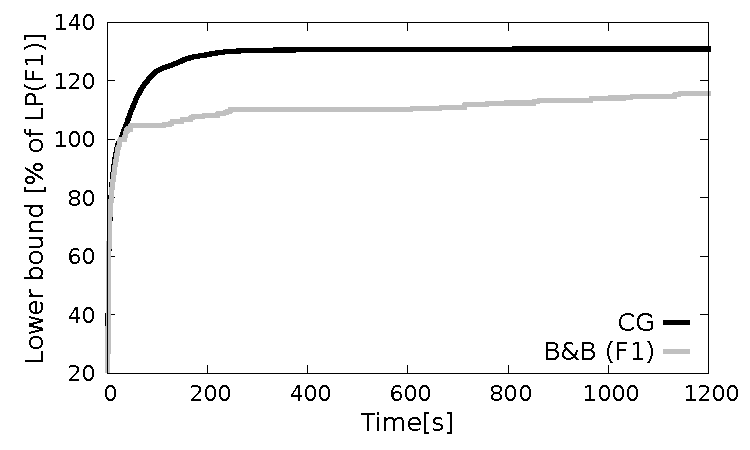
\includegraphics[width=\textwidth]{lower-bound-24-12}
        \caption{$|V|=24, |D|=12$}
        \label{fig:cggr24-12}
    \end{subfigure}
    \hfill %add desired spacing between images, e. g. ~, \quad, \qquad, \hfill etc. 
      %(or a blank line to force the subfigure onto a new line)
    \begin{subfigure}[b]{0.49\textwidth}
        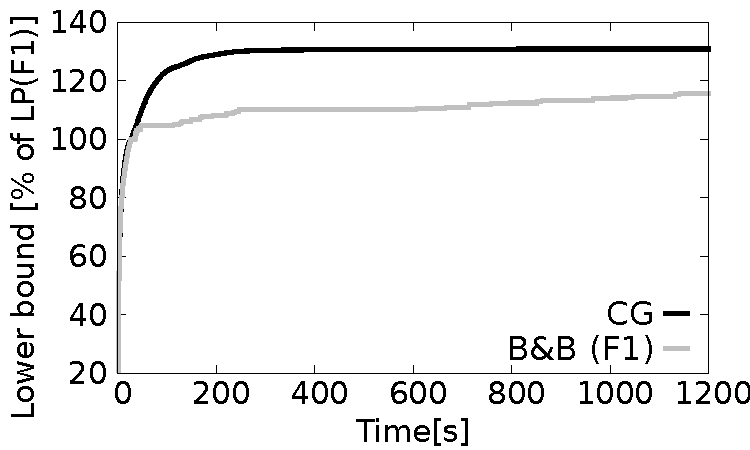
\includegraphics[width=\textwidth]{lower-bound-26-13}
        \caption{$|V|=26, |D|=13$}
        \label{fig:cggr26-13}
    \end{subfigure}
  
    \begin{subfigure}[b]{0.49\textwidth}
        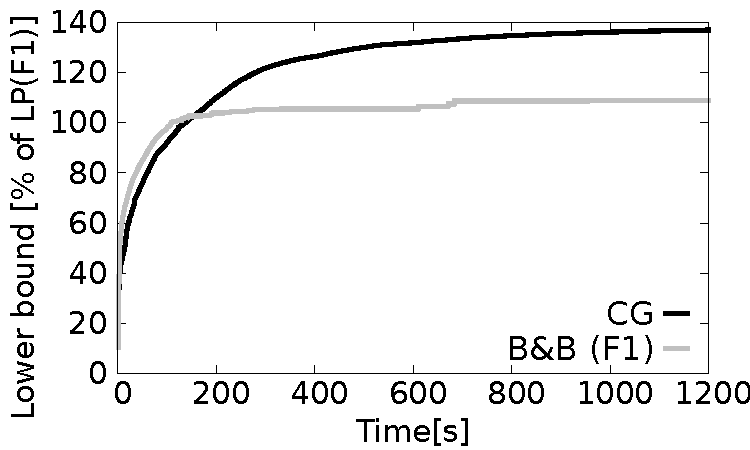
\includegraphics[width=\textwidth]{lower-bound-28-14}
        \caption{$|V|=28, |D|=14$}
        \label{fig:cggr28-14}
    \end{subfigure}
    \hfill %add desired spacing between images, e. g. ~, \quad, \qquad, \hfill etc. 
      %(or a blank line to force the subfigure onto a new line)
    \begin{subfigure}[b]{0.49\textwidth}
        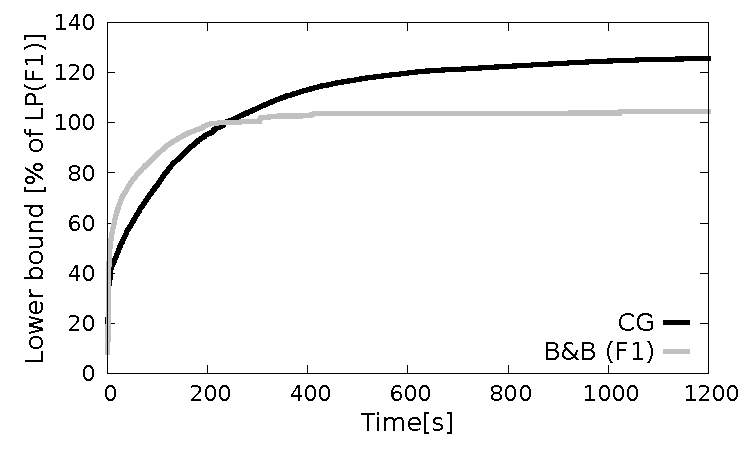
\includegraphics[width=\textwidth]{lower-bound-30-15}
        \caption{$|V|=30, |D|=15$}
        \label{fig:cggr30-15}
    \end{subfigure}

    \begin{subfigure}[b]{0.49\textwidth}
        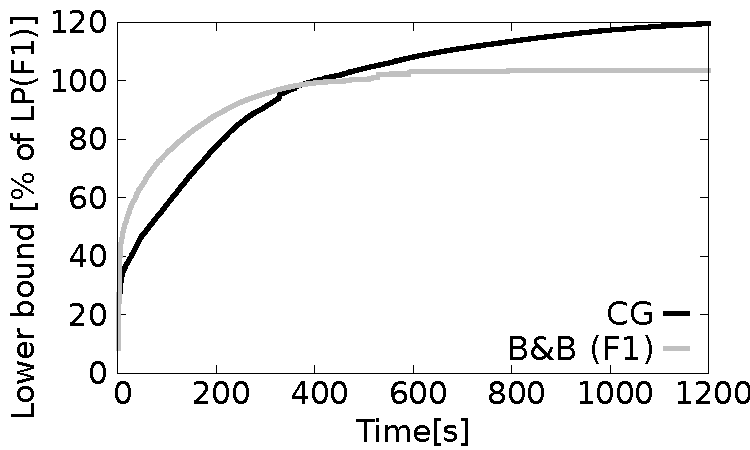
\includegraphics[width=\textwidth]{lower-bound-32-16}
        \caption{$|V|=32, |D|=16$}
        \label{fig:cggr32-16}
    \end{subfigure}
    \hfill %add desired spacing between images, e. g. ~, \quad, \qquad, \hfill etc. 
      %(or a blank line to force the subfigure onto a new line)
    \begin{subfigure}[b]{0.49\textwidth}
        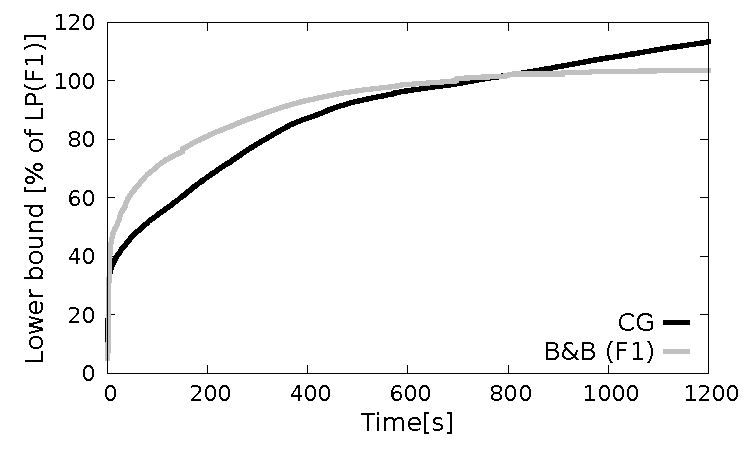
\includegraphics[width=\textwidth]{lower-bound-34-17}
        \caption{$|V|=34, |D|=17$}
        \label{fig:cggr34-17}
    \end{subfigure}
  \caption{Comparison of lower bounds obtained by CG and B\&B on model $\mathcal{F}_1$.
	\textcolor{blue}{Each figure depicts a progress of lower bounds for instances with varying number of destination and non-destination nodes.
	The lower bounds are obtained by solving CG scheme applied on model $\mathcal{F}_1$ (black curves), and produced during the course of classic B\&B algorithm (grey curves)
	The tightness of the bounds increases with time, and it can be observed from the graphs that the CG bound becomes tighter at some point.
	We express the quality of lower bounds with respect to the value of simple continuous relaxation, as indicated by the vertical axes.
	It can also be noted that the lower bound obtained from B\&B grows sharply during the computation of the simplex method in the root of the B\&B tree, 
	which is happening until the curve reaches 100\%.
	After that point the bound grows rather slowly.
	CG on the other hand produces bound that grows faster even after the value of first relaxation in the root is reached.
%	The values can be retrieved from the output of CPLEX during the course of simplex and B\&B algorithm.
	}}
  \label{fig:cggr}
\end{figure} 

Reflecting the progress of the dual simplex method applied to $\text{LP}(\mathcal{X}_2)$ and $\text{LP}(\mathcal{F}_1)$, respectively,
both CG and B\&B increase the lower bound sharply at the beginning. 
While solution of $\text{LP}(\mathcal{F}_1)$ is still in progress, the growth of the lower bound is faster than what is observed for CG (solution of $\text{LP}(\mathcal{F}_1)$). 
This is particularly apparent for instances of size 28 and larger (Fig. \ref{fig:cggr28-14} - \ref{fig:cggr34-17}). %and can be explained as a consequence of Prop. \ref{prop:f1strx1}.
Once $\text{LP}(\mathcal{F}_1)$ is solved, the increase slows down substantially, and remains modest until the time limit is reached. 
An analogous, but more moderate, gradual slow-down is also observed for CG.
In each instance set, the two curves intersect at some point in time.
From this moment on, CG provides a tighter lower bound.
Experiments reported in Fig.\ \ref{fig:cggr} thus indicate that CG is the more suitable method for obtaining tight lower bounds within a given time.

\section{Conclusion and Future Work}
\label{sec:conclusion}
We have presented and analyzed two approaches of modelling the SMT problem as an integer linear program.
The first formulation, $\mathcal{X}_1$, is based on a formulation of the broadcast version of the problem, while the second one, $\mathcal{F}_1$, is an extension of network flow formulation of the minimum Steiner tree problem.
Both formulations are improved by valid inequalities resulting in models $\mathcal{X}_2$ and $\mathcal{F}_2$, respectively. 
Further strengthening is achieved by introducing variables of higher dimension and associated constraints, which leads to models $\mathcal{X}_3$ and $\mathcal{F}_3$.
A theoretical analysis of the formulations shows that  $\mathcal{F}_1$ and $\mathcal{F}_2$ are at least as strong as $\mathcal{X}_1$ and $\mathcal{X}_2$, respectively. 
It is conjectured that an analogous relation holds between $\mathcal{F}_3$ and $\mathcal{X}_3$.
Experimental evaluation reveals that instances with up to approximately 20 nodes are practically solvable to optimality.
Subsequent investigation suggests that the LP relaxations of $\mathcal{F}_3$ and $\mathcal{X}_3$ are fairly strong, but the running time prohibits direct solution.
Nevertheless, experiments also show that a constraint generation procedure applied to $\mathcal{X}_3$, developed in the current work, provides tight lower bounds.
The procedure also demonstrates that when the number of nodes is no more than 30, many instances of the LP relaxation of $\mathcal{X}_3$ have an integer optimum.

Follow-up research should uncover whether the conjecture on the relation between the LP relaxations of $\mathcal{F}_3$ and $\mathcal{X}_3$ holds.
A search for facet-defining valid inequalities, or even convex hull formulations, is an interesting and ambitious direction of future work.
Owing to the limited size of solvable instances, there is a potential in studying inexact methods, such as approximation algorithms and problem specific heuristics.
\textcolor{blue}{In particular, experiments on a simple metaheuristic documented in the current work, suggest that fast and inexact methods have a potential to compute solutions close to optimality in large instances.}
Instance preprocessing combined with variable fixing can possibly increase the size of instances solvable to optimality with the current models.

%We have presented two approaches of modelling SMT as an integer linear program.
%The first formulation is based on broadcast trees, while the second  formulation is an extension of network flow model of the minimum Steiner tree problem.
%Both formulations are improved by valid inequalities and further strengthened by variables of higher dimension and associated constraints.
%A~theoretical analysis reveals that the models based on network flows are at least as strong as the broadcast tree models, with one exception of the strongest extensions of the models, where this claim remains a conjecture.
%Experimental study discovers that practically solvable to optimality are instances with up to approximately 20 nodes.
%Subsequent investigation of LP relaxations suggests that constraint generation applied to the strongest broadcast tree based models is a promising technique for obtaining lower bounds.
%
%%The follow-up research should prove the conjecture that also the strongest network flow based models are at least as strong as the corresponding broadcast tree based models.
%The follow-up research should prove the remaining conjecture regarding relations between the models.
%Additional investigation of facet defining valid inequalities, or even convex hull formulations is a possible direction of future work.
%Owing to the limited size of solvable instances, there is a potential in studying inexact methods such as approximation algorithms and domain specific heuristics.
%Instance preprocessing together with variable fixing could possibly increase the size of instances solvable to optimality with existing models.


%as required. Don't forget to give each section
%and subsection a unique label (see Sect.~\ref{sec:1}).
%\paragraph{Paragraph headings} Use paragraph headings as needed.
%\begin{equation}
%a^2+b^2=c^2
%\end{equation}

% For one-column wide figures use
%\begin{figure}
% Use the relevant command to insert your figure file.
% For example, with the graphicx package use
%  \includegraphics{example.eps}
% figure caption is below the figure
%\caption{Please write your figure caption here}
%\label{fig:1}       % Give a unique label
%\end{figure}
%
% For two-column wide figures use
%\begin{figure*}
% Use the relevant command to insert your figure file.
% For example, with the graphicx package use
%  \includegraphics[width=0.75\textwidth]{example.eps}
% figure caption is below the figure
%\caption{Please write your figure caption here}
%\label{fig:2}       % Give a unique label
%\end{figure*}
%
% For tables use
%\begin{table}
% table caption is above the table
%\caption{Please write your table caption here}
%\label{tab:1}       % Give a unique label
% For LaTeX tables use
%\begin{tabular}{lll}
%\hline\noalign{\smallskip}
%first & second & third  \\
%\noalign{\smallskip}\hline\noalign{\smallskip}
%number & number & number \\
%number & number & number \\
%\noalign{\smallskip}\hline
%\end{tabular}
%\end{table}


%\begin{acknowledgements}
%If you'd like to thank anyone, place your comments here
%and remove the percent signs.
%\end{acknowledgements}

% BibTeX users please use one of
%\bibliographystyle{spbasic}      % basic style, author-year citations
%\bibliographystyle{spmpsci}      % mathematics and physical sciences
%\bibliographystyle{spphys}       % APS-like style for physics
%\bibliography{}   % name your BibTeX data base

% Non-BibTeX users please use
\begin{thebibliography}{}

%
% and use \bibitem to create references. Consult the Instructions
% for authors for reference list style.
%
% \bibitem[Dian{\'e} and Plesn{\'i}k(1993)]{diane93ipf}
% Dian{\'e} M, Plesn{\'i}k J (1993)
% An integer programming formulation of the Steiner problem in graphs.
% Zeitschrift f{\"u}r Operations Research
% 37(1):107--111

\bibitem[Althaus et al.(2003)]{althaus03}
Althaus E, C\u{a}linescu G, M\u{a}ndoiu II, Prasad S, Tchervenski N, Zelikovsky A (2003)
Power efficient range assignment in ad-hoc wireless networks.
In: Proceedings IEEE WCNC’03, pp 1889--1894

\bibitem[Altinkemer et al.(2005)]{altinkemer05}
Altinkemer K, Salman FS, Bellur P (2005)
Solving the minimum energy broadcasting problem in ad hoc wireless networks by integer programming.
In: Proceedings INOC 2005, pp B2.635--B2.642

\bibitem[Bauer et al.(2008)]{bauer08}
Bauer J, Haugland D, Yuan D (2008)
Analysis and computational study of several integer programming formulations for minimum-energy multicasting in wireless ad hoc networks.
Networks 52(2):57–68

\bibitem[Bein and Zheng(2010)]{bein10}
Bein D, Zheng SQ (2010)
Energy efficient all-to-all broadcast in all-wireless networks.
Information Sciences 180(10):1781--1792

\bibitem[Bhukya and Singh(2014)]{bhukya14}
Bhukya WN, Singh A (2014)
\emph{p}-shrink: A Heuristic for Improving Minimum All-to-All Power Broadcast Trees in Wireless Networks.
In: Proceedings of Ninth International Conference on Wireless Communication and Sensor Networks 2014 
Vol.\ 299, pp 61--69

\bibitem[\v{C}agalj et al.(2002)]{cagalj02}
\v{C}agalj M, Hubaux J-P, Enz C (2002)
Minimum-energy broadcast in all-wireless networks: NP-completeness and distribution issues.
In: Proceedings ACM MOBICOM 2002 pp 172--182

\bibitem[Clementi et al.(1999)]{clementi99}
Clementi A, Penna P, Silvestri R (1999)
Hardness results for the power range assignment problem in packet radio networks.
In: Hochbaum D et al. (eds) RANDOM-APPROX’99,
LNCS 1671:197--208

\bibitem[Das et al.(2003)]{das03}
Das AK, Marks RJ, El-Sharkawi M, Arabshani P, Gray A (2003)
Minimum power broadcast trees for wireless networks: integer programming formulations.
In: Proceedings IEEE INFOCOM 2003 Vol.\ 2, pp 1001--1010

\bibitem[Das et al.(2005)]{das05}
Das AK, Marks RJ, El-Sharkawi E, Arabshahi P, Gray A (2005)
Optimization methods for minimum power bidirectional topology construction in wireless networks with sectored antennas.
In: Proceedings IEEE GLOBECOM ’05, pp 3962--3968

\bibitem[Goemans and Myung(1993)]{goemans93catalog}
Goemans MX, Myung Y-S (1993)
A catalog of Steiner tree formulations.
Networks
23(1):19--28

\bibitem[Guo and Yang(2004)]{guo}
Guo S, Yang O (2004)
Minimum Energy Multicast Routing for Wireless Ad-hoc Networks with Adaptive Antennas 
In: Proceedings of the 12th IEEE International Conference on Network Protocols ICNP 2004,
pp 151--160

\bibitem[Halgamuge et al.(2009)]{halgamuge}
Halgamuge MN, Zukerman M, Ramamohanarao K (2009)
An estimation of sensor energy consumption.
Progress In Electromagnetics Research B 12:259--295

\bibitem[Haugland and Yuan(2011)]{Haugland11Compact}
Haugland D, Yuan D (2011)
Compact integer programming models for power-optimal trees in ad hoc wireless networks.
In: Kennington J, Olinick E, Rajan D (eds) Wireless network design - optimization models and solution procedure.
International series in operations research \& management science.
Springer, New York, pp 219--246

\bibitem[Hsiao et al.(2013)]{hsiao13}
Hsiao P-C, Chiang T-C, Fu L-C (2013)
Static and dynamic minimum energy broadcast problem in wireless ad-hoc networks: A PSO-based approach and analysis
Applied Soft Computing
13:786--4801

\bibitem[Ivanova(2016)]{ivanova16isco}
Ivanova M (2016)
Shared Multicast Trees in Ad Hoc Wireless Networks.
In: Cerulli R, Fujishige S, Mahjoub A (eds) Combinatorial Optimization ISCO 2016,
LNCS 9849:273--284

\bibitem[Kirousis et al.(1997)]{kirousis97}
Kirousis LM, Kranakis E, Krizanc D, Pelc A (1997)
Power consumption in packet radio networks.
In: Reischuk M (ed): STACS'97 Proceedings,
LNCS 1200:363--374

\bibitem[Leggieri et al.(2008)]{leggieri08}
Leggieri V, Nobili P, Triki C (2008)
Minimum power multicasting problem in wireless networks.
Math Meth Oper Res 68:295–311

\bibitem[Montemanni and Gambardella(2004)]{montemanni04}
Montemanni R, Gambardella LM (2004)
Exact algorithms for the minimum power symmetric connectivity problem in wireless networks.
Comput Oper Res 31(10):1667--1680

\bibitem[Montemanni and Leggieri(2011)]{montemanni11}
Montemanni R, Leggieri V (2011)
A branch and price algorithm for the minimum power multicasting problem in wireless sensor networks.
Math Meth Oper Res
74:327--342

\bibitem[Pajor et al.(2018)]{pajor18}
Pajor T, Uchoa E, Werneck RF (2018)
A robust and scalable algorithm for the Steiner problem in graphs.
Math Prog Comp 10:69--118

\bibitem[Papadimitriou and Georgiadis(2006)]{Papadimitriou06SBT}
Papadimitriou I, Georgiadis L (2006)
Minimum-energy Broadcasting in Multi-hop Wireless Networks Using a Single Broadcast Tree.
Mobile Netw Appl
11(3):361--375

\bibitem[Polzin and Daneshmand(2001)]{Polzin}
Polzin T, Daneshmand SV (2001)
A comparison of Steiner tree relaxations.
Discrete Appl Math
112(1--3):241--261

\bibitem[Wieselthier et al.(2000)]{Wieseltier00onthe}
Wieselthier JE, Nguyen GD, Ephremides A (2000)
On the Construction of Energy-Efficient Broadcast and Multicast Trees in Wireless Networks,
In: Proceedings IEEE INFOCOM 2000 Vol.\ 2, pp 585--594

\bibitem[Yuan(2005)]{yuan05}
Yuan D (2005)
An integer programming approach for the minimum-energy broadcast problem in wireless networks.
In: Proceedings INOC 2005, pp B2.643–B2.650

\bibitem[Yuan et al.(2008)]{yuan08}
Yuan D, Bauer J, Haugland D (2008)
Minimum-energy broadcast and multicast in wireless networks: An
integer programming approach and improved heuristic algorithms.
Ad Hoc Netw
6(5):696–717

\bibitem[Yuan and Haugland(2012)]{Haugland12Dual}
Yuan D, Haugland D (2012)
Dual Decomposition for Computational Optimization of Minimum-Power Shared Broadcast Tree in Wireless Networks.
IEEE T Mobile Comput
12(11):2008--2019

%\bibitem{RefJ}
% Format for Journal Reference
%Author, Article title, Journal, Volume, page numbers (year)
% Format for books
%\bibitem{RefB}
%Author, Book title, page numbers. Publisher, place (year)
% etc
\end{thebibliography}

\end{document}
% end of file template.tex

